%%%%%%%%%%%%%%%%%%%%%%%%%%%%%%%%%%%%%%%%%%%%%%%%%%%%%%%%%%%%%%%%%%%%%%%%%%%%%%%%
%2345678901234567890123456789012345678901234567890123456789012345678901234567890
%        1         2         3         4         5         6         7         8

\documentclass[letterpaper, 10 pt, conference]{ieeeconf}  % Comment this line out if you need a4paper
% \documentclass[conference]{IEEEtran}

% \documentclass[a4paper, 10pt, conference]{ieeeconf}      % Use this line for a4 paper

\IEEEoverridecommandlockouts                              % This command is only needed if 

\overrideIEEEmargins                                      % Needed to meet printer requirements.

\usepackage{amsmath,amssymb,amsfonts}
\usepackage{tikz}                                                          % you want to use the \thanks command
\usepackage[T1]{fontenc}
\usepackage[utf8]{inputenc}
\usepackage{xcolor,colortbl}
\usepackage{subcaption}
\graphicspath{ {images/} } 
\usepackage{blindtext}
\usepackage{subfiles}
\usepackage{algorithm}
\usepackage{algpseudocode}
\usepackage{multicol}
% \usepackage{float}
\usepackage{stfloats}
\usepackage{array}
%\usepackage[maxfloats=256]{morefloats}
%\maxdeadcycles=15000
\usepackage{url}
\usepackage{diagbox}
\usepackage{flushend}
\usepackage{lipsum}
\usepackage[verbose]{placeins} 
\usepackage{multirow}
\usepackage{subcaption}
\newtheorem{lemma}{Lemma}
\newcolumntype{C}[1]{>{\centering\arraybackslash}p{#1}}
\newcolumntype{M}[1]{>{\centering\arraybackslash}m{#1}}
\let\labelindent\relax  % Redefine before loading enumitem
\usepackage{enumitem}
\newcommand{\purplecircle}{\textcolor{blue}{\textbullet}}
\newcommand{\largepurplecircle}{\textcolor{blue}{\scalebox{1.5}{$\bullet$}}}
\newcommand{\CRD}{$\text{C}_{\text{R}} \text{D }$}
\newcommand{\problemtitle}[2]{%
  \parbox{\linewidth}{\centering\textbf{#1} \\ \textbf{#2}}%
}
\newtheorem{problem}{Problem}
%\newcommand{\DoTikzmark}[1]{%
%  \tikz[remember picture] \coordinate[shift={(0,.7ex)}](#1);%
%}
%\newcommand{\colrow}[3][]{%
%  \tikz[overlay,remember picture, line width=10pt]
%    \draw[shorten >=-.1em, shorten <=-.1em, #1] (#2)--(#3);
%}

%\newcommand{\mc}[2]{\multicolumn{#1}{c}{#2}}
%\definecolor{Gray}{gray}{0.85}
%\definecolor{LightCyan}{rgb}{0.88,1,1}

%\newcolumntype{a}{>{\columncolor{Gray}}c}
%\newcolumntype{b}{>{\columncolor{white}}c}

%\newenvironment{remark}{
%  \par\medskip
%  \noindent\textbf{\textcolor{blue}{Remark.}} \ignorespaces
%  \color{red}\itshape
%}{
%  \par\medskip
%}








%In case you encounter the following error:
%Error 1010 The PDF file may be corrupt (unable to open PDF file) OR
%Error 1000 An error occurred while parsing a contents stream. Unable to analyze the PDF file.
%This is a known problem with pdfLaTeX conversion filter. The file cannot be opened with acrobat reader
%Please use one of the alternatives below to circumvent this error by uncommenting one or the other
%\pdfobjcompresslevel=0
%\pdfminorversion=4

% See the \addtolength command later in the file to balance the column lengths
% on the last page of the document

% The following packages can be found on http:\\www.ctan.org
%\usepackage{graphics} % for pdf, bitmapped graphics files
%\usepackage{epsfig} % for postscript graphics files
%\usepackage{mathptmx} % assumes new font selection scheme installed
%\usepackage{times} % assumes new font selection scheme installed
%\usepackage{amsmath} % assumes amsmath package installed
%\usepackage{amssymb}  % assumes amsmath package installed

\title{\LARGE \bf Improving Urban Cycling Safety and Comfort\\ through Optimized Infrastructure Upgrades   }
%Graph-Metric to Asses Safety/Stress in Large-Scale Bike Mobility Networks
% \author{Manuel Campero Jurado, Mauro Salazar, Giovanni De Nunzio, Carlos Canudas-de-Wit}
\author{Manuel Campero Jurado$^{1}$, Mauro Salazar$^{2}$, Giovanni De Nunzio$^{3}$, Carlos Canudas-de-Wit$^{1}$% <-this % stops a space
%\thanks{*This work was not supported by any organization}% <-this % stops a space
\thanks{$^{1}$Univ. Grenoble Alpes, Inria, CNRS, Grenoble INP, GIPSA-Lab, 38000 Grenoble, France
        {\footnotesize \{\textit{manuel.campero-jurado@inria.fr, carlos.canudas-de-wit@gipsa-lab.fr}\} }}%
\thanks{$^{2}$Eindhoven University of Technology, 5600 MB, Eindhoven, The Netherlands
        {\footnotesize \{\textit{m.r.u.salazar@tue.nl\}}}}%
\thanks{$^{3}$IFP Energies nouvelles,
Rond-point de l’échangeur de Solaize, BP 3, 69360 Solaize, France,
        {\footnotesize \textit{\{giovanni.de-nunzio@ifpen.fr\}}}}%
% \thanks{$^{4}$Univ. Grenoble Alpes, CNRS, Inria, Grenoble INP, GIPSA-lab, 11 Rue des Mathématiques, 
% 38400 Saint-Martin-d'Hères-Grenoble-France
        % {\footnotesize carlos.canudas-de-wit@gipsa-lab.fr}}%
}



\begin{document}
\pagestyle{empty}


\maketitle
% \thispagestyle{plain}
% \pagestyle{plain}


%%%%%%%%%%%%%%%%%%%%%%%%%%%%%%%%%%%%%%%%%%%%%%%%%%%%%%%%%%%%%%%%%%%%%%%%%%%%%%%%
\begin{abstract}

% This paper presents a bi-level optimization framework to enhance urban cycling infrastructure by strategically upgrading the bike lanes degree of separation (DoS) from motorized traffic. The DoS classification, with six levels, reflects increasing safety and comfort as cyclists' exposure to annual average daily traffic decreases. The lower level of the framework estimates cyclist flows using an all-or-nothing assignment method that incorporates factors such as slope, angular changes, and cars traffic, providing a realistic flow distribution across the network. At the upper level, the optimization problem seeks to minimize cyclists' traffic exposure by upgrading segments to higher DoS levels within a fixed budget. We present a case study of Grenoble's cycling network, applying this framework with a modified genetic algorithm to optimize safety, comfort, and budget efficiency. The results are compared to those of a specialized algorithm designed to enhance overall perceived safety and comfort across the network. Findings demonstrate that targeted infrastructure upgrades significantly improve local and overall safety and comfort, and promote a more balanced distribution of cyclist flows. This approach offers urban planners a practical tool for prioritizing investments in cycling infrastructure.

% This paper introduces a bi-level optimization framework to improve urban cycling infrastructure by upgrading bike lanes' degree of separation (DoS) from motorized traffic. The lower level estimates cyclist flows using an all-or-nothing assignment, while the upper level minimizes traffic exposure by optimizing DoS upgrades within a fixed budget. Applied to Grenoble’s cycling network, the framework uses a modified genetic algorithm to enhance safety, comfort, and budget efficiency. Results show that targeted upgrades improve both local and overall safety, balance cyclist flows, and provide a practical tool for urban planners to prioritize infrastructure investments.

This paper proposes a bi-level optimization framework to improve urban cycling infrastructure by upgrading bike lanes' degree of separation from motorized traffic. The six-level degree of separation classification reflects increasing safety and comfort as cyclists' exposure to annual average daily traffic decreases. The lower level estimates cyclist flows using an all-or-nothing assignment method that accounts for factors like slope, angular changes, and traffic, ensuring realistic flow distribution. The upper level minimizes traffic exposure by upgrading segments to higher DoS levels within a fixed budget. A case study on Grenoble's cycling network applies this framework using a modified genetic algorithm to optimize safety, comfort, and budget efficiency. Results are compared to a specialized algorithm designed to improve overall perceived safety and comfort. Findings highlight that targeted infrastructure upgrades enhance both local and network-wide safety, better balancing cyclist flows. This framework provides urban planners with a data-driven tool for prioritizing cycling infrastructure investments.


\end{abstract}

\begin{keywords}
Cycling infrastructure, bi-level optimization, degree of separation, annual average daily traffic, safety, comfort, urban planning.
\end{keywords}


%%%%%%%%%%%%%%%%%%%%%%%%%%%%%%%%%%%%%%%%%%%%%%%%%%%%%%%%%%%%%%%%%%%%%%%%%%%%%%%%
\section{Introduction}
% Cycling offers numerous health, environmental, and socioeconomic benefits, such as improved cardiovascular health, increased longevity, reduced carbon emissions, lower transportation costs, and reduced traffic congestion \cite{garrard2012health, krizec2007estimating, gotschi2016cycling}. Recognizing these advantages, public authorities have actively promoted cycling as a sustainable alternative to short-distance car travel. However, the decision to ride a bicycle often depends on safety and comfort perceived factors \cite{fishman2012barriers}. Research consistently shows that separating bike lanes from motorized traffic improves cyclists’ perceptions of safety and comfort, encouraging higher ridership \cite{lawrence2018cyclist, broach2012cyclists}. High-quality, connected cycling infrastructure further amplifies these benefits, with studies indicating strong potential for increased cycling when cohesive, secure facilities are available \cite{pucher2011walking, pucher2017cycling}. Therefore, given budget limitations, cities must strategically prioritize cycling infrastructure investments to maximize cyclist safety and comfort. Effective planning is essential to allocate resources where they will have the greatest impact.

% \textit{Related Work:} The dynamics of bicycle flow and optimization of cycling infrastructure have received considerable attention in recent literature. In \cite{mesbah2012bilevel, smith2012mathematical}, bi-level optimization approaches are used to maximize cycling distances while minimizing car travel times, balancing benefits for both cyclists and motorists. Additionally, \cite{paulsen2023societally} evaluates gradual network expansions through societal cost-benefit analyses.

% Graph-theoretic optimization techniques have also been applied to enhance cycling network connectivity that aims to improve cyclist experience. For example, \cite{duthie2014optimization} presents a framework that minimizes upgrade costs by prioritizing connectivity, ensuring that all origin-destination pairs for cyclists are accessible via routes that meet a specified level of service. Similarly, \cite{mauttone2017bicycle} proposes an optimization model that balances shorter routes with budget constraints. In \cite{cooper2017using}, an all-or-nothing bicycle traffic assignment approach is applied to model cyclist flows, considering factors like slope and angular changes.

% While existing methods provide useful insights, they generally do not prioritize cyclist comfort and safety through targeted infrastructure upgrades. Our framework fills this gap with a bi-level approach: the upper level strategically upgrades bike lanes to reduce cyclists' exposure to traffic, taking into account infrastructure costs and lane characteristics, while the lower level evaluates how these upgrades affect cyclist flow distributions. This approach captures the interdependent effects of safety, comfort, and flow dynamics—an integrated framework that, to the best of our knowledge, has not been previously developed.

% \textit{Statement of Contributions:} This paper proposes a modeling and  bi-level optimization framework for upgrading cycling infrastructure based on a six-category classification of bike lanes by degree of separation (DoS) from motor traffic. Higher DoS levels correspond to greater safety and comfort, reducing exposure to car traffic. Our framework focuses on upgrading lanes from lower to higher DoS categories to maximize cyclist comfort and safety. Key contributions include: (1) estimating cyclist flows with an all-or-nothing assignment method that incorporates factors like slope, angular changes, and AADT; (2) formulating a bi-level optimization problem from a utilitarian perspective to minimize cyclists' exposure to traffic, while accounting for the redistribution of flows due to infrastructure upgrades, as applied to the Grenoble cycling network; and (3) to solve the problem, we modify a standard genetic algorithm aiming at budget efficiency to achieve a balanced solution that respects budget constraints. We then compare its results with those of an algorithm specifically designed to improve overall perceived safety and comfort by maximizing the largest connected component (CC) \cite{2024graphbased}.

% \textit{Organization:} The remainder of this paper is organized as follows: Section \ref{osm_data} describes the data sources and the bike lane classification. Section \ref{model_design} details the model design, including the flow assignment method, the bi-level optimization problem, the algorithms used to address it and introduce the largest CC metric to assess the perceived safety and comfort on the network in order to validate our results. Section \ref{study_case} presents a case study of the Grenoble cycling network. Section~\ref{conclusions} concludes the paper and outlines directions for future research.

Cycling provides significant health, environmental, and economic benefits, including improved cardiovascular health, lower emissions, and reduced congestion \cite{garrard2012health, krizec2007estimating, gotschi2016cycling}. To encourage cycling, authorities promote it as an alternative to short-distance car travel. However, perceived safety and comfort strongly influence ridership \cite{fishman2012barriers}. Studies show that physically separated lanes enhance safety perception, boosting cycling rates \cite{lawrence2018cyclist, broach2012cyclists}. Well-connected, high-quality infrastructure further increases cycling adoption \cite{pucher2011walking, pucher2017cycling}. Given budget constraints, cities must strategically invest in infrastructure to maximize safety and comfort where it has the greatest impact.

\textit{Related Work:} The dynamics of bicycle flow and optimization of cycling infrastructure have received considerable attention in recent literature. In \cite{mesbah2012bilevel, smith2012mathematical}, bi-level optimization approaches are used to maximize cycling distances while minimizing car travel times, balancing benefits for both cyclists and motorists. Additionally, \cite{paulsen2023societally} evaluates gradual network expansions through societal cost-benefit analyses.

\begin{figure}[t]
    \centering
% 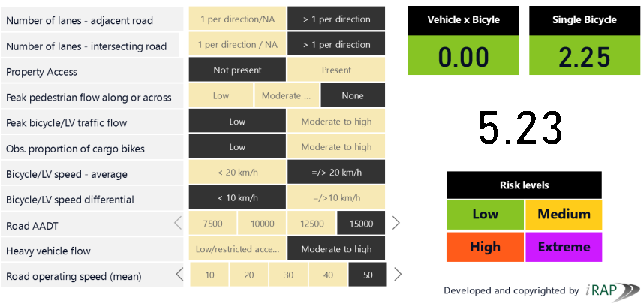
\includegraphics[width=\columnwidth]{Images/cyclerap.pdf}
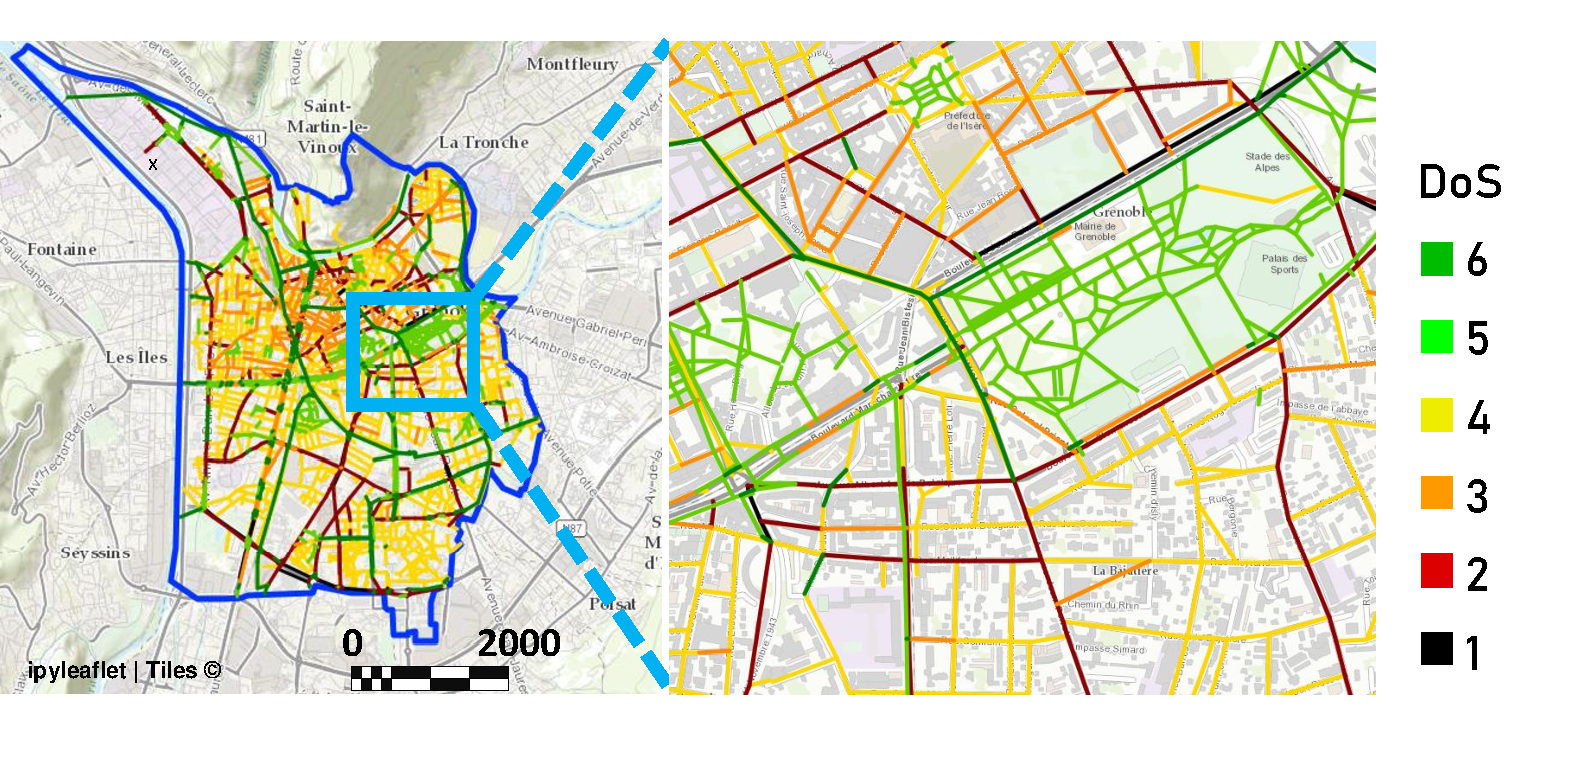
\includegraphics[width=\columnwidth]{Images/Map_and_scale.pdf}
    \caption{\footnotesize Cycling network of Grenoble, France. The degree of separation (DoS) score of the cycling infrastructure from motorized vehicles is indicated in ascending order from 1 to 6.}
    \label{networks_classification}
\end{figure}

Graph-theory optimization techniques have also been applied to enhance cycling network connectivity that aims to improve cyclist experience. For example, \cite{duthie2014optimization} presents a framework that minimizes upgrade costs by prioritizing connectivity, ensuring that all origin-destination pairs for cyclists are accessible via routes that meet a specified level of service. Similarly, \cite{mauttone2017bicycle} proposes an optimization model that balances shorter routes with budget constraints. In \cite{cooper2017using}, an all-or-nothing bicycle traffic assignment approach is applied to model cyclist flows, considering factors like slope and angular changes.

While existing methods provide useful insights, they generally do not prioritize cyclist comfort and safety through targeted infrastructure upgrades. Our framework fills this gap with a bi-level approach: the upper level strategically upgrades bike lanes to reduce cyclists' exposure to traffic, taking into account infrastructure costs and lane characteristics, while the lower level evaluates how these upgrades affect cyclist flow distributions. This approach captures the interdependent effects of safety, comfort, and flow dynamics—an integrated framework that, to the best of our knowledge, has not been previously developed.

\textit{Statement of Contributions:} This paper proposes a modeling and  bi-level optimization framework for upgrading cycling infrastructure based on a six-category classification of bike lanes by degree of separation (DoS) from motor traffic. Higher DoS levels correspond to greater safety and comfort, reducing exposure to car traffic. Our framework focuses on upgrading lanes from lower to higher DoS categories to maximize cyclist comfort and safety. Key contributions include: (1) estimating cyclist flows with an all-or-nothing assignment method that incorporates factors like slope, angular changes, and annual average daily traffic (AADT); (2) formulating a bi-level optimization problem from a utilitarian perspective to minimize cyclists' exposure to traffic, while accounting for the redistribution of flows due to infrastructure upgrades, as applied to the Grenoble cycling network; and (3) to solve the problem, we modify a standard genetic algorithm aiming at budget efficiency to achieve a balanced solution that respects budget constraints. We then compare its results with those of an algorithm specifically designed to improve overall perceived safety and comfort by maximizing the largest connected component (CC) \cite{2024graphbased}.

\textit{Organization:} The remainder of this paper is organized as follows: Section \ref{osm_data} describes the classification of bike lanes and the graph representation of the network. Section \ref{model_design} details the model design, including the flow assignment method, the bi-level optimization problem, the algorithms used to address it. Section \ref{study_case} presents a case study of the Grenoble cycling network. Section~\ref{conclusions} concludes the paper and outlines directions for future research.


%%%%%%%%%%%%%%%%%%%%%%%%%
\section{Network Data and Features}
\label{osm_data}

% In this section, we describe the construction of the cycling network employing a six-category classification based on DoS. These scores are used as weights for the links in the mathematical graph representing the cycling network and establish the classification order, which will serve as a reference for modeling the improvement of moving from one category to a safer and more comfortable higher level category.

This section outlines the construction of the cycling network using a six-category DoS classification. These scores serve as link weights in the network graph and define the hierarchy for modeling upgrades to safer and more comfortable categories.


\subsection{Bike Lane Classification}
%The DoS categories are adapted from Geovelo\footnote{\url{https://gitlab.com/geovelo-public/requetes_amenagements_cyclables/-/tree/master}}, a platform that classifies bike lanes into twenty-two types using OpenStreetMap (OSM) data. Following the method in \cite{2024graphbased}, these classifications are simplified into six primary DoS categories, emphasizing physical separation from motor traffic to represent various levels of safety and comfort \cite{nolan2021bicycle}. The classification methodology is publicly available\footnote{\url{https://github.com/leunamCampero/ITSC2024}}. The classification system used here combines DoS categories with additional metrics such as annual average daily traffic (AADT), speed limits, and the number of bike lanes to provide a more accurate measure of perceived safety and comfort across different cycling routes. This integrated measure, that enhances the traditional DoS framework by incorporating key traffic characteristics.

% Adapted from Geovelo's platform, which uses OpenStreetMap (OSM) data to classify bike lanes, the DoS categories are simplified into six main levels to reflect varying safety and comfort based on physical separation from traffic \cite{2024graphbased}. The methodology is publicly available online\footnote{\url{https://github.com/leunamCampero/ITSC2024}}.
% Table~\ref{dos_table} presents the DoS categories, along with their alignment with the Geovelo classification, where numbers are assigned based on alphabetical sorting. High-DoS lanes (DoS 6 and 5) maintain the best scores regardless of annual average daily traffic (AADT), given their full separation from motor traffic. In contrast, low-DoS lanes experience reduced safety and comfort as AADT increases. Fig.~\ref{networks_classification} visualizes the classifications in the city of Grenoble, France.

Based on Geovelo's platform, which classifies bike lanes using OpenStreetMap (OSM) data, the DoS categories are condensed into six levels to represent safety and comfort variations according to physical separation from traffic \cite{2024graphbased}. The methodology is openly available online\footnote{\url{https://github.com/leunamCampero/ITSC2024}}. Table~\ref{dos_table} outlines the DoS categories and their correspondence with Geovelo’s classification, where numbers are assigned alphabetically. High-DoS lanes (DoS 6 and 5) consistently achieve the highest safety and comfort scores due to full separation from motor traffic, while lower-DoS lanes become less safe and comfortable as AADT increases. Fig.~\ref{networks_classification} illustrates these classifications in Grenoble, France.

% From this point forward, whenever we mention or assume a change in the DoS, we are referring to a change its corresponding CycleRAP score. For example, when we state that a road is upgraded from DoS 5 to DoS 6, we mean that its score changes from 4.64 to 5.23.

% \begin{figure}[t]
%     \centering
% 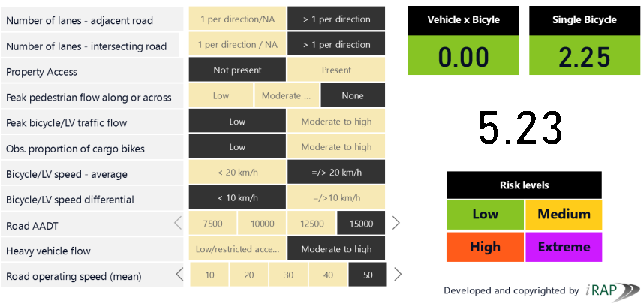
\includegraphics[width=\columnwidth]{Images/cyclerap.pdf}
%     \caption{ CycleRAP demonstrator tool for scoring cycling facilities.}
%     \label{cycle_rap}
% \end{figure}




% \begin{figure}[t]
%     \centering
% 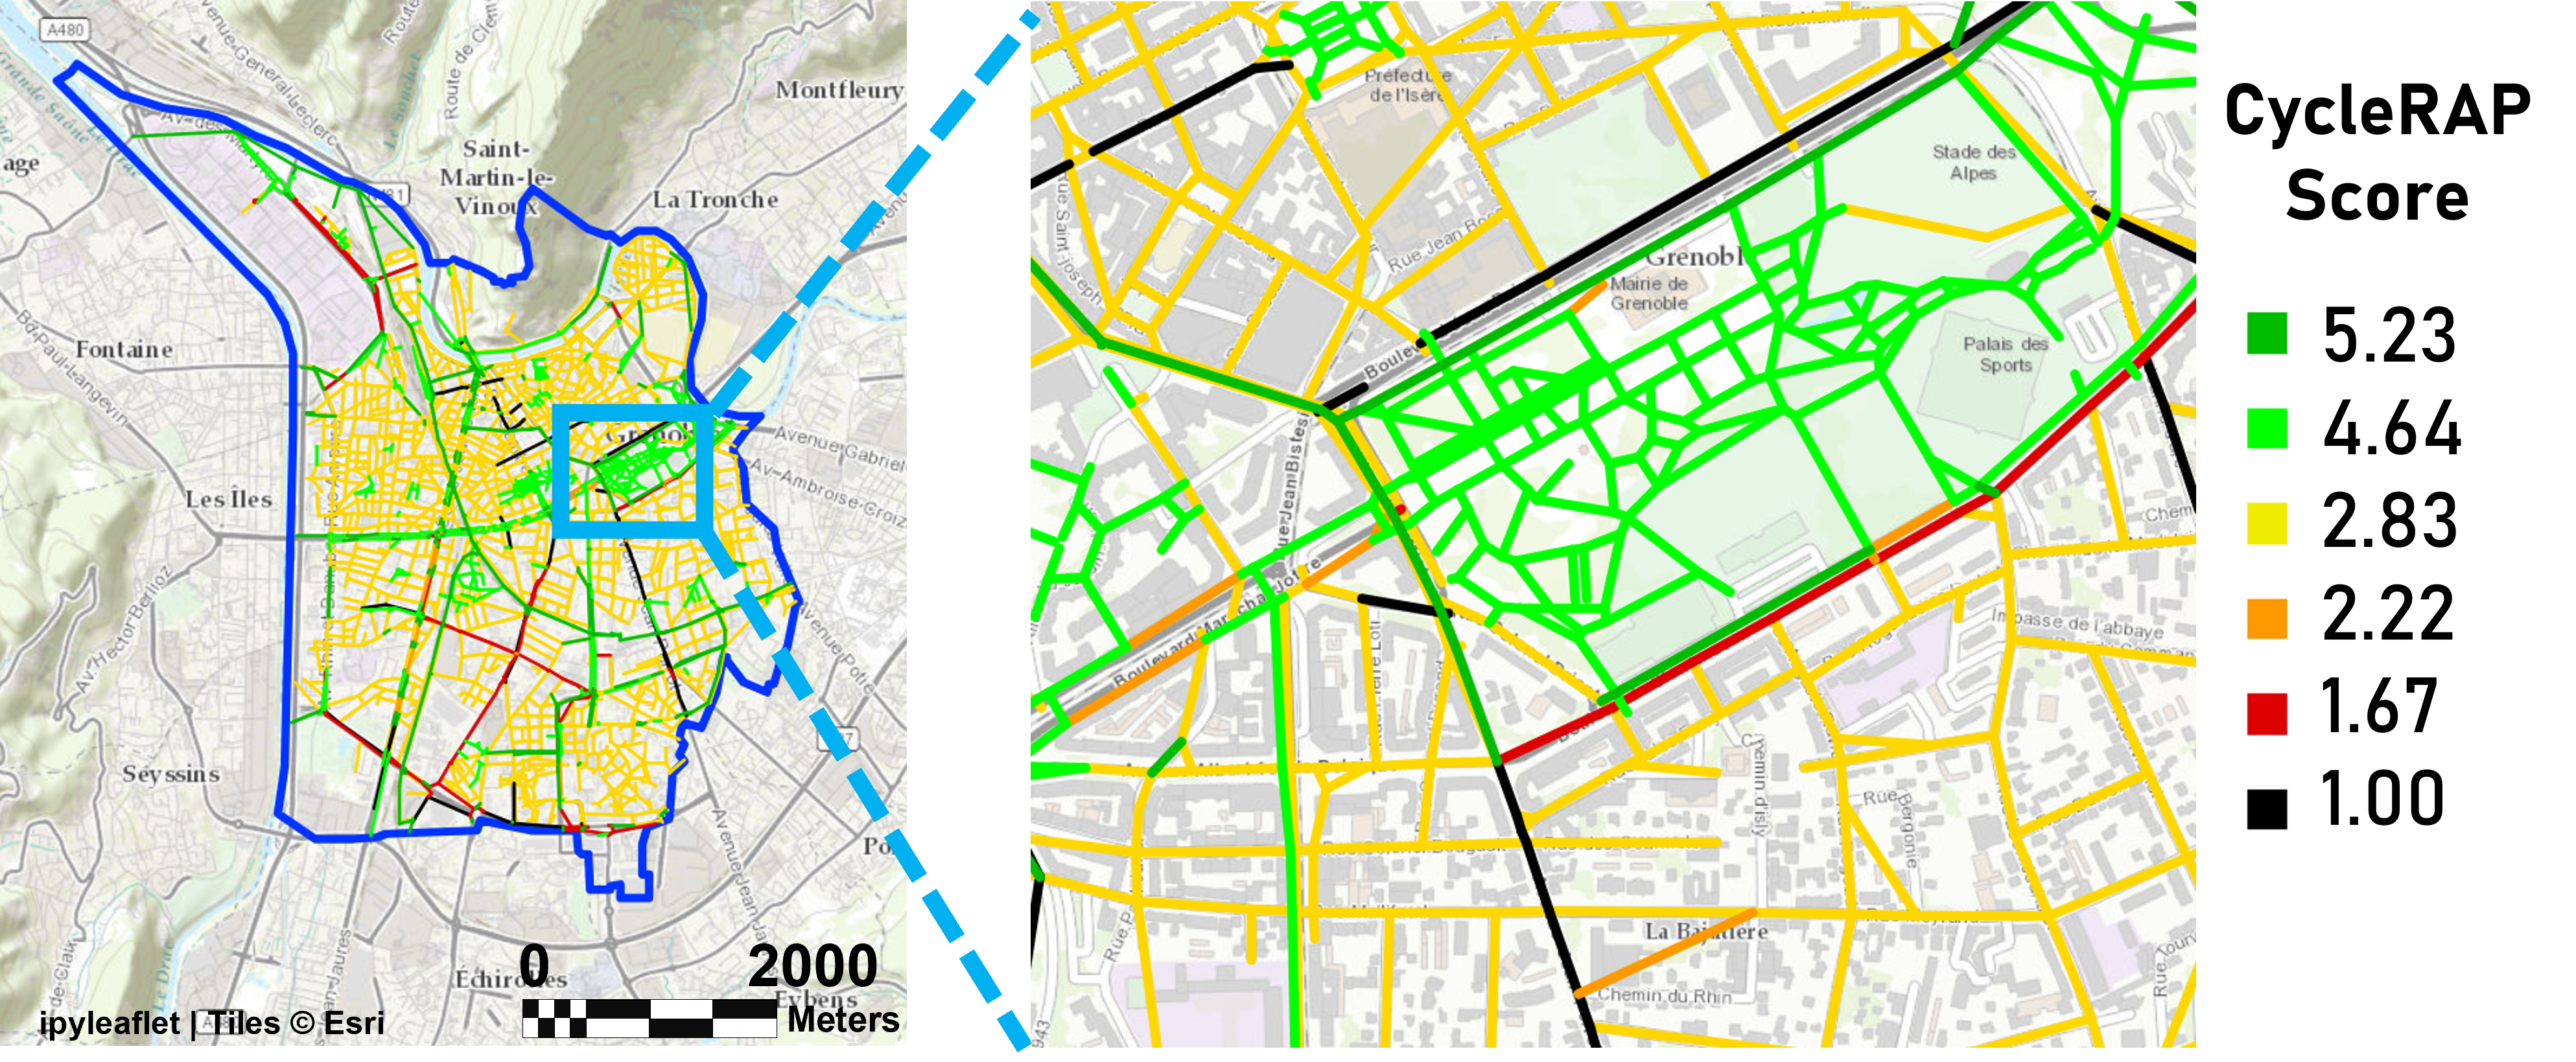
\includegraphics[width=\columnwidth]{Images/map_scale.png}
%     \caption{ Cycling network of Grenoble, France. The CycleRAP score of the cycling infrastructure from motorized vehicles is indicated in ascending order from 1 to 5.23.}
%     \label{networks_classification}
% \end{figure}




\begin{table*}[t]
\centering
\vspace{0.2cm}
\begin{tabular}{|>{\centering\arraybackslash}p{0.02\linewidth}|p{0.40\linewidth}|>{\centering\arraybackslash}p{0.18\linewidth}|C{0.13\linewidth}|C{0.14\linewidth}|}
\hline
\textbf{DoS}   & \textbf{Description} & \textbf{Geovelo} & \textbf{AADT (veh/day)} & \textbf{Mean speed (km/hr)} \\
\hline
 $6$ & Dedicated bike lanes, fully separated from motor traffic. & 7, 14 & 14 400 & 50 \\

$5$  & Bike lanes shared with pedestrians, separate from cars. & 2, 10, 11, 15, 16, 17, 20 & 16 000 & 50 \\ 
$4$  & Mixed-traffic roads (30 km/h) without designated bike lanes. & 9, 12, 13, 21, 22 & 960 & 30  \\

$3$  & Shared roads with cycling pictograms. & 5, 8 & 3 120 & 30 \\

$2$  & Roads with painted bike lanes. & 1, 3, 4, 6 & 6 912 & 40  \\

$1$  & Unmarked shared car-bike lanes. & 18, 19 & 8 448 & 40  \\
\hline



\end{tabular}
\caption{\footnotesize The first column represents the degree of separation (DoS), which categorizes bike lane infrastructure based on safety levels. The second column describes the category of cycling infrastructure. The third column lists the corresponding Geovelo classification numbers. The fourth and fifth columns present data from the GTLVille platform in Grenoble, detailing annual average daily traffic (AADT) and car mean speed in the adjacent roads to cycling paths, respectively.}
\label{dos_table}
\end{table*}

% \begin{table}[h!]
% \centering
% \begin{tabular}{|l|p{2cm}|p{1.5cm}|l|}
% \hline
% \textbf{Source Name} & \textbf{Function} & \textbf{Data Type} & \textbf{Reference} \\ \hline
% Geovelo             & Categorizes bike lanes by separation level & Infrastructure classification & \cite{2024graphbased} \\ \hline
% CycleRAP            & Provides crash risk scores & Safety and comfort scoring & \cite{cyclerap2024} \\ \hline
% GTLVille            & Estimates AADT and mean speed near bike paths & Traffic and speed data & \cite{gtlville2024} \\ \hline
% EMD2020             & Surveys general mobility patterns & Household mobility data & \cite{SMMAG_EMD} \\ \hline
% Cerema              & Provides bicycle trip distribution based on distance & Mode choice probability & \cite{cerema2024mobility} \\ \hline
% \end{tabular}
% \caption{\footnotesize Summary of data sources used in the cycling network model. All the data used is openly accessible.}
% \label{table:data_sources}
% \end{table}
\subsection{Graph Representation}

Let the network be represented by a weighted directed graph (digraph) $\mathcal{G} = (\mathcal{V}, \mathcal{A}, \mathcal{W})$, where $\mathcal{V}$ is the set of nodes corresponding to intersections or road endpoints, $\mathcal{A}$ is the set of directed arcs representing roads, and $\mathcal{W}$ is the set of weights assigned to those arcs. For each arc $a = (u, v) \in \mathcal{A}$, with $u,v \in \mathcal{V}$, the weight $w_a \in \mathcal{W}$ represents the DoS associated with the link. The weights are assumed to be symmetric, meaning $w_{(u,v)} = w_{(v,u)}$. The geographical length of each arc $a$ is denoted by $d_a$.

% In \cite{2024graphbased}, the authors proved that the DoS category effectively model layers that align with safety and comfort perceptions. Then, moving arcs from one DoS level to a higher one locally enhance safety and comfort by reducing traffic exposure, thereby encouraging flow distribution onto higher DoS roads. Ultimately, this approach translates into improved overall safety and comfort across the network.
In \cite{2024graphbased}, the authors demonstrated that the DoS classification effectively represents safety and comfort perceptions. Upgrading arcs to higher DoS levels locally enhances safety by reducing traffic exposure, encouraging cyclists to shift toward safer routes. This, in turn, leads to improved overall safety and comfort across the network.

\section{Model Design}
\label{model_design}
In this section, we introduce the model for predicting cyclist flows, followed by the bi-level optimization problem, which aims to minimize cyclists' exposure to traffic while accounting for the distribution of cycling flows across the network to improve safety and comfort.  Finally, we then present the two algorithms employed to solve this NP-hard problem. 

% \subsection{Demand distribution}
% \begin{figure}[t]
%     \centering
% 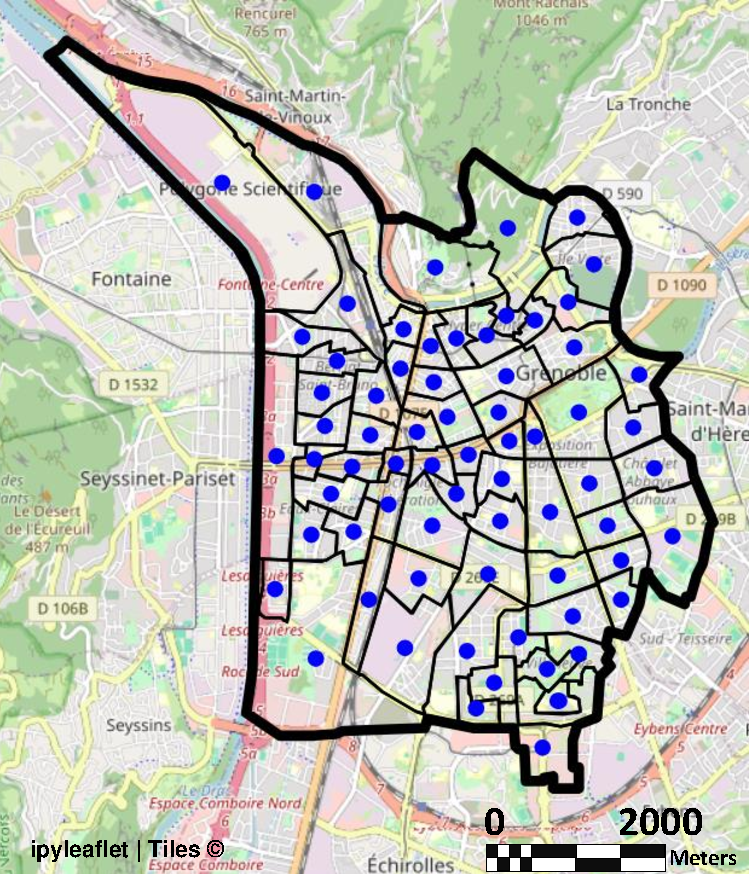
\includegraphics[width=0.65\columnwidth]{Images/Grenoble_od.pdf}
% % \includegraphics[width=1.1\columnwidth]{Images/Grenoble_poverty_rate.pdf}
%     \caption{\footnotesize Layout of Grenoble city. \largepurplecircle{} Blue circles represent OD centroids of the regions.}
%     \label{o_d_centrodis}
% \end{figure}

%%%%%%%%%%%%%%%%%%%%%%%%%%%%%%%%%%%%%%%%%%%%%%%%%%%%%%%%%%%%%%%%%%%%%%%%%%%%%%%%%%%%%%%%%%%%%%%%%%%%%%%%%%
% From the EMD2020 household survey \cite{SMMAG_EMD} we obtain general mobility data (a summary of the data sources used in this work are included in Table \ref{table:data_sources}), clustered at the centroids of Grenoble's regions as shown in Fig. \ref{o_d_centrodis}. To distribute this demand across all nodes in the cycling network, we follow the approach in \cite{mehrotra2022revisiting}, which applies graph theory metrics for resource allocation. This method considers the distance of network nodes to resource sources. In this context, the resource source is defined as the largest CC, where each arc within the component has the highest possible DoS $=6$. This component is denoted by $\mathcal{C}$ representing the largest portion of the network with the highest level of safety and comfort.
% %This approach aligns with Rawls' difference principle \cite{rawls1971theory}, ensuring fair distribution by giving higher weights to nodes farther from fully safe and comfortable areas, thus enhancing accessibility for those with less connectivity.

% For each node $v \in \mathcal{V}$, define $d_{\mathcal{C}}(v)$ as the shortest geographical distance to the nearest node of $\mathcal{C}$. To normalize distances, we define
% \begin{equation}
%     c(v) = \frac{d_{\mathcal{C}}(v)}{\max_{\tilde{v} \in \mathcal{V}} d_{\mathcal{C}}(\tilde{v})} \in [0, 1],
% \end{equation}
% which represents the normalized closeness of node $v$ to $\mathcal{C}$, with values closer to 1 indicating less proximity to fully safe areas.

% Let $\mathcal{R} = \{1, \ldots, R\}$ denote the regions in Grenoble, where each region $r \in \mathcal{R}$ has a node $v_r \in \mathcal{V}$ representing the aggregated origin/destination (OD) point. For each pair $(r, s) \in \mathcal{R} \times \mathcal{R}$, $q_{(r, s)}$ represents the global mobility demand from region $r$ to region $s$.

% Let $\mathcal{V}^{r} \subseteq \mathcal{V}$ be the nodes in region $r$. The regional demand $q_{(r, s)}$ is distributed among nodes $v \in \mathcal{V}^{r}$ and $u \in \mathcal{V}^{s}$ as follows:
% \begin{equation}
%     \bar{q}_{(u, v)} = q_{(r, s)} \cdot \frac{c(v)}{\sum_{\tilde{v} \in \mathcal{V}^{r}} c(\tilde{v})} \cdot \frac{c(u)}{\sum_{\tilde{u} \in \mathcal{V}^{s}} c(\tilde{u})}.
% \end{equation}
% This allocation is symmetric:
% \begin{equation}
%     \bar{q}_{(u, v)} = \bar{q}_{(v, u)} \forall v, u \in \mathcal{V}.
% \end{equation}

% Next, to allocate trips specifically to cycling, we draw on Cerema’s data regarding bicycle trip distribution \cite{cerema2024mobility}. For each OD pair $(u, v)$, multiply the total trips $\bar{q}_{(u,v)}$ by the probability $\mathbb{P} = 0.05$ to estimate the number of bicycle trips $q_{(u,v)}$ as follows:
% \begin{equation}
%     q_{(u,v)} = \bar{q}_{(u,v)} \cdot \mathbb{P}_{\text{bike}}.
% \end{equation}
% Then, $q_{(u,v)}$ represents the number of cyclists traveling from node $u$ to node $v$.
%    % \begin{equation}
%    % \mathbb{P}_{\text{bike}}(d_{u,v}) = 
%    % \begin{cases} 
%    %    0.20 & \text{if } d_{u,v} < 1 \text{ km} \\
%    %    0.50 & \text{if } 1 \leq d_{u,v} < 2 \text{ km} \\
%    %    0.17 & \text{if } 2 \leq d_{u,v} < 5 \text{ km} \\
%    %    0.10 & \text{if } 5 \leq d_{u,v} < 10 \text{ km} \\
%    %    0.03 & \text{if } d_{u,v} \geq 10 \text{ km}
%    % \end{cases}
%    % \label{tab:bike_prob}
%    % \end{equation}
% % \begin{table}[h!]
% % \centering
% % \begin{tabular}{c|c}
% % \hline
% % Distance Range $d_{(u,v)}$ (km) & $\mathbb{P}_{\text{bike}}(d_{(u,v)})$ \\ \hline
% % $d_{(u,v)} < 1$ & 0.20 \\ 
% % $1 \leq d_{(u,v)} < 2$ & 0.50 \\ 
% % $2 \leq d_{(u,v)} < 5$ & 0.17 \\ 
% % $5 \leq d_{(u,v)} < 10$ & 0.10 \\ 
% % $d_{(u,v)} \geq 10$ & 0.03 \\ \hline 
% % \end{tabular}
% % \caption{Probability of choosing cycling based on geographical distance.}
% % \label{tab:bike_prob}
% % \end{table}







%%%%%%%%%%%%%%%%%%%%%%%%%%%%%%%%%%%%%%%%%%%%%%%%%%%%%%%%%%%%%%%%%%%%%%%%%%%%%%%%%%%%%%%%%%%%%%%%%%%%%%%%%%

%%%%%%%%%%%%%%%%%%%%%%%%%%%%%%%%%%%%%%%%%%%%%%%%%%%%%%%%%%%%%%%%%%%%%%%%%%%%%%%%%%%%%%%%%%%%%%%%%%%%%%%%%%
\subsection{Cyclist Flows}
\label{section_flows}
%%%%%%%%%%%%%%%%%%%%%%%%%%%%%%%%%%%%%%%%%%%%%%%%%%%%%%%%%%%%%%%%%%%%%%%%%%%%%%%%%%%%%%%%%%%%%%%%%%%%%%%%%%
% \begin{table*}[h!]
% \centering
% \begin{tabular}{|c|l|c|c|}
% \hline
% \textbf{Symbol} & \textbf{Description} & \textbf{Domain} & \textbf{Unit} \\ \hline
% $u, v$ & Nodes in the cycling network & $\mathcal{V}$ & - \\ \hline
% $p_{(u,v)}$ & Shortest path between nodes $u$ and $v$ & $\mathcal{P}$ & - \\ \hline
% $d_{a}$ & Geographical length of arc $a$ & $\mathbb{R}_{>0}$ & meters \\ \hline
% $\measuredangle_{a}$ & Angular change at arc $a$ (junctions) & $\mathbb{R}$ & degrees \\ \hline
% $s_{a}$ & Slope factor based on terrain slope & $\mathbb{R}_{\geq 0}$ & - \\ \hline
% $f_{a}$ & Traffic factor reflecting car traffic impact & $\mathbb{R}_{\geq 0}$ & - \\ \hline
% $b_{(u,v)}$ & Modified cyclist distance between nodes $u$ and $v$ & $\mathbb{R}_{\geq 0}$ & meters \\ \hline
% $\sigma_{u,v}^{b}$ & Total shortest paths between $u$ and $v$ based on $b$ & $\mathbb{N}$ & - \\ \hline
% $\sigma_{u,v}^{b}(a)$ & Shortest paths traversing arc $a$ between $u$ and $v$ & $\mathbb{N}$ & - \\ \hline
% $B_{a}$ & Betweenness centrality of arc $a$ & $\mathbb{R}_{\geq 0}$ & - \\ \hline
% $Q$ & Aggregated demand across all nodes in the network & $\mathbb{R}_{\geq 0}$ & - \\ \hline
% $x_{a}$ & Flow on arc $a$ & $\mathbb{R}_{\geq 0}$ & - \\ \hline
% $\alpha, \beta$ & Model calibration parameters & $\mathbb{R}$ & - \\ \hline
% $\text{AADT}$ & Annual Average Daily Traffic on arc $a$ & $\mathbb{R}_{\geq 0}$ & vehicles/day \\ \hline
% $\text{DoS}(a)$ & Degree of Separation on arc $a$ & $\{1,2, \ldots,6\}$ & - \\ \hline
% $\theta^{\star}$ & Parameters in network-upgrade optimization & $\mathbb{R}^{4}$ & - \\ \hline
% $w_{a}$ & Original weight for arc $a$ & $\mathbb{N}$ & - \\ \hline
% $\tilde{w}_{a}$ & Candidate weight for arc $a$ (optimized) & $\mathbb{N}$ & - \\ \hline
% $\pi(w_{a},\tilde{w}_{a})$ & Cost per meter of upgrading arc $a$ & $\mathbb{R}_{\geq 0}$ & currency/meter \\ \hline
% $l_{\mathcal{G}_{\tilde{w}}}$ & Total length of modified network with $\tilde{w}$ & $\mathbb{R}_{\geq 0}$ & meters \\ \hline
% $t_{(u,v)}$ & Travel time between $u$ and $v$ & $\mathbb{R}_{\geq 0}$ & minutes \\ \hline
% $t_{\text{max}}$ & Time threshold for accessibility & $\mathbb{R}_{>0}$ & minutes \\ \hline
% \end{tabular}
% \caption{Summary of Notation for Core Variables in Cycling Network Model}
% \label{table:notation_summary}
% \end{table*}

\begin{table}[h!]
\centering
\vspace{0.2cm}
\begin{tabular}{|c|l|c|c|}
\hline
\textbf{Symbol} & \textbf{Description} & \textbf{Domain} & \textbf{Unit} \\ \hline
$q_{(u,v)}$ & Bike demand from $u$ to $v$ & $\mathbb{R}_{\geq 0}$ & bike/day \\
$p_{(u,v)}$ & Shortest path between $u$ and $v$ & $\mathcal{A}$ & - \\ 
$d_{a}$ & Arc $a$ length/distance & $\mathbb{R}_{>0}$ & m \\ 
$\measuredangle_{a}$ & Angular change at $a$ & $\mathbb{R}_{\geq 0}$ & deg \\ 
$s_{a}$ & Slope factor of arc $a$ & $\mathbb{R}_{\geq 0}$ & - \\ 
$f_{a}$ & Traffic factor on arc $a$ & $\mathbb{R}_{\geq 0}$ & - \\ 
$b_{(u,v)}$ & Cyclist distance $u$-$v$ & $\mathbb{R}_{\geq 0}$ & m \\ 
$x_{a}$ & Flow on arc $a$ & $\mathbb{R}_{\geq 0}$ & bike/day \\ 
$x_{p}$ & Flow on path $p$ & $\mathbb{R}_{\geq 0}$ & bike/day \\ 
$\sigma_{p_{(u,v)}}(a)$ & arc $a$ is part of shortest path $p$? & $ \left\{ 0,1\right\}$ & - \\ 
$\rho, \kappa, \psi$ & Calibration parameters & $\mathbb{R}$ & - \\ 
$x^{\text{AADT}}_{a}$ & AADT adjacent to $a$ & $\mathbb{R}_{\geq 0}$ & veh/day \\ 
$w_{a}$ & Original DoS of $a$ & $\mathbb{R}_{\geq 0}$ & - \\ 
$\tilde{w}_{a}$ & Candidate DoS for $a$ & $\mathbb{R}_{\geq 0}$ & - \\ 
$\pi(w_{a},\tilde{w}_{a})$ & Upgrade cost for $a$ & $\mathbb{R}_{\geq 0}$ & € \\ 
$J_{\mathcal{E}}$ & Total cyclist exposure & $\mathbb{R}_{\geq 0}$ & -\\
\hline
\end{tabular}
\caption{\footnotesize Abbreviated notation for variables in cycling network model.}
\label{table:notation_summary}
\end{table}

% In \cite{mesbah2012bilevel}, a traffic assignment problem for bicycles is formulated. While this model assumes possible congestion, if we do not account for congestion, we can instead use an all-or-nothing assignment based on the shortest path, as done in \cite{cooper2018predictive, cooper2017using}, which we adopt in this section. These works use OpenStreetMap and pedal cycle flow data from Cardiff, UK, to calibrate parameters for predicting cyclist flows on links. They define a distance metric that considers cycling infrastructure and apply betweenness centrality to predict flows across the network.

% Following \cite{mesbah2012bilevel}, we use an all-or-nothing (AON) traffic assignment model that assumes no congestion and assigns all demand $q_{(u,v)}$ from the EMD2020 survey \cite{SMMAG_EMD} to the shortest available path  between nodes $u,v \in \mathcal{V}$. In \cite{mesbah2012bilevel}, it is demonstrated that an all-or-nothing traffic assignment model for bicycles is feasible under the assumption of no congestion, where essentially all demand \( q_{(u,v)} \) between nodes \( u \) and \( v \) is assigned to the shortest path connecting them. This approach simplifies the flow assignment by relying on the shortest path, as implemented in \cite{cooper2017using} and adopted here. This study employs OpenStreetMap and cycling flow data from Cardiff, UK, to calibrate parameters for predicting cyclist flows along network links. It then defines a custom distance metric that incorporates cycling infrastructure characteristics and, a betweenness centrality metric is applied to estimate the flow distribution across the cycling network. The method is formally presented below.

Following \cite{mesbah2012bilevel}, we use an all-or-nothing (AON) traffic assignment model under the assumption of no congestion, where all demand $q_{(u,v)}$ from the EMD2020 survey \cite{SMMAG_EMD} is assigned to the shortest available path between nodes $u,v~\in~\mathcal{V}$. This approach, demonstrated in \cite{mesbah2012bilevel} and implemented in \cite{cooper2017using}, simplifies flow assignment by prioritizing the shortest path. Additionally, OpenStreetMap and cycling flow data from Cardiff, UK, are used to calibrate parameters, define a custom distance metric incorporating cycling infrastructure, and apply betweenness centrality to estimate flow distribution. The method is formally presented below.



% To account for factors specific to cycling, we define a modified distance metric. Let \( u, v \in \mathcal{V} \), and let \( p^{(u,v)} = (a_{1},\ldots, a_{k}) \) represent a shortest path between nodes \( u \) and \( v \). For an arc \( a \in p^{(u,v)} \), let \( d_{a} \) denote the geographical length, \( \theta_{a} \) the angular change in degrees (either along \( a \) or at junctions between consecutive arcs), \( s_{a} \) the slope factor, which is determined by the terrain slope \( m_{a} \), and \( f_{a} \) the traffic factor, which accounts for traffic conditions. We define the cyclist distance \( b_{(u,v)} \) between nodes \( u \) and \( v \) as:
To incorporate cycling-specific factors,a modified distance metric is defined. Let $u, v \in \mathcal{V}$ be nodes, and let $p_{(u,v)}~=~(a_{1}, \ldots, a_{k})$ represent the shortest path between $u$ and $v$. For an arc $a \in p_{(u,v)}$, let $d_{a}$ denote the geographical length; $\measuredangle_{a}$ represents the angular change (in degrees) along $a$ if it is the first or last arc in the path, or at junctions between consecutive arcs; $s_{a}$ the slope factor based on the terrain slope $m_{a}$; and $f_{a}$ the traffic factor, representing car traffic conditions on roads adjacent to bike lanes, which can significantly impact bike flow on lanes that are shared with car traffic.

The cyclist distance $b_{(u,v)}$ between nodes $u$ and $v$ is then defined as
\begin{equation}
\label{cyclist_distance}
    b_{(u,v)} = \sum_{a \in p_{(u,v)}} \left( d_{a} \cdot s_{a} \cdot (f_{a})^{\rho} \right) +  \sum_{a \in p_{(u,v)}} \measuredangle_{a} \cdot \kappa.
\end{equation}

% The slope factor $s_{a}$ is determined as follows. For uphill travel ($m_{a} \geq 0$), we use:
% \begin{equation}
% s_{a} = h_{a} = 
% \begin{cases}
% 1.0 & \text{if } m_{a} < 2, \\
% 1.371 & \text{if } 2 \leq m_{a} < 4, \\
% 2.203 & \text{if } 4 \leq m_{a} < 6, \\
% 4.239 & \text{if } m_{a} \geq 6.
% \end{cases}    
% \end{equation}
The traffic factor $f_{a}$ is defined as
\begin{equation}
\label{f_a}
f_{a} = 
     \begin{cases}
\psi \cdot \exp{\left( x^{\text{AADT}}_{a} \right)} & \text{if } w_{a} < 5, \\
\psi \cdot 2.03 & w_{a} = 5, \\
\psi & w_{a} = 6,
\end{cases}
\end{equation}
% \begin{table}[h!]
% \centering
% \begin{tabular}{c|c|c}
% \hline
% Slope ($m_a$) \% & Uphill Factor ($s_a$) & Downhill Factor ($s_a$) \\ \hline
% $m_a < 2$ & 1.0 & 1.0 \\ 
% $2 \leq m_a < 4$ & 1.371 & $1/1.371 \approx 0.729$ \\ 
% $4 \leq m_a < 6$ & 2.203 & $1/2.203 \approx 0.454$ \\ 
% $m_a \geq 6$ & 4.239 & $1/4.239 \approx 0.236$ \\ \hline
% \end{tabular}
% \caption{Slope Factors for Cycling Distance Calculation}
% \label{table:slope_factors}
% \end{table}


% For downhill travel ($m_{a} < 0$), the slope factor is reduced to account for lower effort:

% \begin{equation}
%     s_{a} = \frac{1}{h_{a}}.
% \end{equation}
% Alternatively, this can be presented in Table \ref{tab:slope_factors}.

% \begin{table}[h!]
% \centering
% \caption{Slope Factor \( sm_{a} \) based on Terrain Slope \( m_{a} \)}
% \label{tab:slope_factors}
% \begin{tabular}{c|c}
% \hline
% Terrain Slope \( m_{a} \) & Slope Factor \( sm_{a} \) \\
% \hline
% \( m_{a} < 2 \) & 1.0 \\
% \( 2 \leq m_{a} < 4 \) & 1.371 \\
% \( 4 \leq m_{a} < 6 \) & 2.203 \\
% \( m_{a} \geq 6 \) & 4.239 \\
% \hline
% \end{tabular}
% \end{table}






where $x^{\text{AADT}}_{a}$ and $w_{a}$ represent the annual average daily traffic of the car lanes adjacent to bike arc $a$ expressed in $1000$s, and the DoS for bike arc $a$, respectively. According to \cite{cyclerap2024}, the effect of AADT is neutralized if the cycling lane is fully separated from car lanes (i.e., when $\text{DoS} = 5$ or $6$). The factor of 2.03 signifies more than twice the probability of bike crash risk in spaces shared with pedestrians compared to fully separated infrastructure, as identified in \cite{mesimaki2021near}.


Let $p_{(u,v)}$ be the shortest path between nodes $u$ and $v$ based on the cyclist distance in \eqref{cyclist_distance}. Since the origin-destination (OD) demand in our data is symmetric, each node acts as both an origin and a destination, ensuring balanced inflow and outflow. The flow conservation for paths is given by

\begin{equation}
\label{eq_shortest_path}
    x_{p_{(u,v)}} = q_{(u,v)},
\end{equation}

where $q_{(u,v)}$ represents the demand between nodes $u$ and $v$. Next, let $\sigma_{p_{(u,v)}}(a)$ be a binary variable indicating whether arc $a$ is part of the shortest path $p_{(u,v)}$. Then, the total cyclist flow on arc $a$, denoted as $x_a$, is

\begin{equation}
\label{eq_flows}
  x_{a} = \sum_{u,v \in \mathcal{V}} q_{(u,v)} \cdot \sigma_{p_{(u,v)}}(a) \geq 0, \quad \forall a \in \mathcal{A}.
\end{equation}
This ensures that the total flow on each arc is the sum of all demands for trips passing through it, maintaining balance across the network due to the symmetry of the demand matrix.

To assess cyclist exposure to traffic conditions, we introduce $\mathcal{E}$ as a general measure of exposure, defined for pahts in the network. This metric helps evaluate network improvements. For a shortest path $p_{(u,v)} = (a_1, \dots, a_k)$, cyclist exposure captures the combined effect of traffic-related risk and the distance of cyclist interaction with traffic, and is defined as
\begin{equation}
\label{exposure_def}
    \mathcal{E}_{p_{(u,v)}} = \sum_{a \in p_{(u,v)}} d_{a} \cdot f_{a},
\end{equation}
where $d_{a}$ and $f_{a}$ are the normalized arc length and traffic factor, respectively. For a single arc $a \in \mathcal{A}$, cyclist exposure simplifies to
\begin{equation}
\label{arc_exposure}
    \mathcal{E}_{a} = d_{a} \cdot f_{a} \in  \left [ 0,1 \right ].
\end{equation}

Next, we introduce the bi-level optimization frameworks for improving cyclist safety. The lower-level problem estimates cyclist flows via AON assignment, incorporating slope and traffic factors. The upper-level optimization selects lane upgrades to reduce cyclist exposure while incorporating both utilitarian and sufficientarian transport justice principles. Additionally, we introduce the algorithms designed to solve these problems efficiently.



%  Each upgrade of the cycling infrastructure (i.e., increasing the DoS value of a road segment or arc) incurs a cost per meter. The DoS values can transition from any value to any equal or greater value, with the requirement that these upgrades remain discrete. Our objective is to optimize the selection of arcs to be upgraded in order to minimize the flow in links with low DoS of a specific cycling network $\mathcal{G}$ within a fixed budget $B$. We introduce the following notations:
% \begin{itemize}
%     \item $w_{0} = \left [ w_{1}, \ldots, w_{a}, \ldots, w_{|\mathcal{A}|} \right ]$ are the original arc weights \CRD of the graph $\mathcal{G}$ to be optimized.
%     \item $\tilde w = \left [ \tilde{w}_{1},  \ldots, \tilde{w}_{a}, \ldots,\tilde{w}_{|\mathcal{A}|} \right ] \in \Omega $ are the candidate weights to be optimized, with,
%     \begin{equation} \nonumber
%         \Omega = \left \{ \tilde{w} \in \mathbb{N}^{|\mathcal{A}|} \colon w_{a} \leq \tilde{w}_{a} \leq w_{\text{DoS}_{6}},  \forall a \in \left \{1, \ldots, |\mathcal{A}| \right \}  \right\}.
%     \end{equation} 
%     \item $f =  \left [ x_{1}^{\text{AADT}}, \cdots, x_{a}^{\text{AADT}}, \cdots, x_{|\mathcal{A}|}^{\text{AADT}} \right ]$ the vector with the average daily traffic of each arc as defined in eq. \ref{f_a}.
%     \item $b = \left [ b_{1}, \cdots, b_{a}, \cdots, b_{|\mathcal{A}|} \right ]$ vector of the length of the arcs according to cyclist distance as in eq. \ref{cyclist_distance}.
    
% \end{itemize}
% Then the optimization problem is defined as bilevel optimization problem where the upper level is:
% \noindent\textbf{Problem: Upgrade DoS-Flows-Cyclist distance}
% \begin{align}
%     \label{problem_a_1}
%      & \; \underset{\tilde{\omega} \in \Omega}{\operatorname{argmin}} \; f^\top x^{\star} \\
%     & \label{problem_a_3} \text{under} \quad   \sum_{a=1}^{|\mathcal{A}|} d_{a} \cdot \pi(w_{a},\tilde{w}_{a}) \leq B.
% \end{align}
% And the lower part is:
% \begin{align}
%     \label{problem_a_1}
%     x^{\star} &= \; \underset{\tilde{\omega} \in \Omega}{\operatorname{argmax}} \; b(\cdot, f)^\topx \\
%     & \label{problem_a_3} \text{under} 
%     \sum_{p \in \mathcal{P}_{(u,v)}} x_{(u,v)}^{p} = q_{(u,v)}.\\
%     & \quad \quad  x_{(u,v)}^{p} \geq 0, \quad \forall u,v \in \mathcal{V}.
% \end{align}


%%%%%%%%%%%%%%%%%%%%%%%%%%%%%%%%%%%%%%%%%%%%%%%%%%%%%%%%%%%%%%%%%%%%%%%%%%%%%%%%%%%%%%%%%%%%%%%%%%%%%%%%%%
\subsection{Optimization Problem}
\label{optimization_problem}
Taking a utilitarian perspective, we aim to reduce cyclists' average exposure to vehicular traffic while accounting for their flow distribution across the network. By prioritizing upgrades that enhance the DoS within a fixed budget $B$, we seek to maximize the average safety and comfort of cyclists, directing flows toward safer routes and reducing high-traffic exposure for all network users.

Each upgrade to the cycling infrastructure, such as increasing a road segment’s DoS, incurs a cost per meter. DoS upgrades are discrete and must satisfy a fixed budget $B$. We define the following notations:

\begin{itemize}
    \item $\mathbf{w}_{0} = \left [ w_{1}, \ldots, w_{a}, \ldots, w_{|\mathcal{A}|} \right ]^\top \in \mathbb{N}^{|\mathcal{A}|}$: the original arc weights (DoS) of the graph $\mathcal{G}$;
    \item $\tilde{\mathbf{w}} = \left [ \tilde{w}_{1}, \ldots, \tilde{w}_{a}, \ldots, \tilde{w}_{|\mathcal{A}|} \right ]^\top \in \Omega$: the candidate weights to be optimized, whereby
\end{itemize}

\begin{equation}
\Omega = \left \{ \tilde{w} \in \mathbb{N}^{|\mathcal{A}|} \colon w_{a} \leq \tilde{w}_{a} \leq 6,  \forall a \in \{1, \ldots, |\mathcal{A}| \} \right\};    
\end{equation}

Additionally, we define the following, where the values are normalized to be scaled between their respective minimum and maximum values:

\begin{itemize}
    \item $\mathbf{b}(\tilde{\mathbf{w}}) = \left [ b_{1}, \cdots, b_{a}, \cdots, b_{|\mathcal{A}|} \right ]^\top \in \mathbb{R}^{|\mathcal{A}|}_{\geq 0}$: the vector of normalized  cyclist distances, defined in~\eqref{cyclist_distance};
    \item $\mathbf{x}^\star(\tilde{\mathbf{w}}) = \left [ x_{1}, \cdots, x_{a}, \cdots, x_{|\mathcal{A}|} \right ]^\top \in \mathbb{R}^{|\mathcal{A}|}_{\geq 0}$: the vector of normalized arc flows resulting from the AON assignment, computed according to~\eqref{eq_shortest_path} and~\eqref{eq_flows};
    \item $\boldsymbol{\mathcal{E}}(\tilde{\mathbf{w}}) = \left [ \mathcal{E}_{1}, \cdots, \mathcal{E}_{a}, \cdots, \mathcal{E}_{|\mathcal{A}|} \right ]^\top \in \mathbb{R}^{|\mathcal{A}|}_{\geq 0}$: the vector of traffic exposure, which is also a function of the chosen upgrades $\tilde{\mathbf{w}}$, as defined in~\eqref{arc_exposure};
    \item $\pi(w_{a},\tilde{w}_{a}) \in \mathbb{R}_{\geq 0}$: the cost per meter of upgrading arc $a$ from its original DoS $w_{a}$ to the new DoS $\tilde{w}_{a}$;
    \item $J_{\mathcal{E}} = \boldsymbol{\mathcal{E}}^\top(\tilde{\mathbf{w}}) \mathbf{x}^\star(\tilde{\mathbf{w}}) \in \mathbb{R}_{\geq 0}$: the total cyclist exposure throughout the network, where both $\boldsymbol{\mathcal{E}}$ and $\mathbf{x}^{\star}$ depend on the chosen DoS levels $\tilde{\mathbf{w}}$.
    %This objective corresponds to the utilitarian perspective, as it aims to maximize overall safety improvements across the network. 
\end{itemize}

% For the bilevel optimization problem the upper-level problem focuses on strategically upgrading cycling infrastructure to minimize cyclist exposure to traffic. The upper-level solution ensures that resources are allocated to improve paths with the highest cyclist flows (optimized for comfort) and traffic exposure. The model prioritizes improvements on routes where the minimized cycling effort (from the lower-level solution) intersects with high vehicle traffic, achieving the greatest safety benefit for cyclists within budget constraints. 
The optimization problem has two interconnected levels:

\textit{Upper-Level Problem} ($\mathbb{U}$): This problem represents the strategic infrastructure planning goal. Here, we aim to minimize cyclist exposure to car traffic by choosing optimal upgrades to the DoS across the network, while staying within the budget $B$. The objective function minimizes the total exposure defined as the product of arc length, traffic factor, and cyclist flow. This ensures that upgrades prioritize long arcs with high traffic factors and flows, as they present the greatest risk of exposure to cyclists.

\textit{Lower-Level Problem} ($\mathbb{L}$): This problem represents the flow distribution, which models how cyclists will travel across the network once the upgrades have been made. The objective is to determine the optimal distribution of cyclist flows across the network by assigning each origin-destination (OD) pair to the path that minimizes cyclist distance by an all-or-nothing assignment as in Section~\ref{section_flows}. This distribution depends on the cyclist-specific distance metric, which reflects the comfort and safety of each route.

Because changes in the DoS at the upper level influence the cyclist distance (and thus the flows) at the lower level, the two levels are nested. This means that every decision made at the upper level affects the solution of the lower level. 
% In this bi-level optimization problem, our goal is to strategically upgrade cycling infrastructure to minimize cyclist exposure to traffic, as determined by the degree of separation (DoS) in Eq. (\ref{f_a}). The upgrades optimize for both safety and comfort, while staying within budget constraints that is our upper level ($\mathbb{P}_{1}$). But this is a nested problem where each change in the DoS may make a change in the flows. So the objective is to minimize the "effort" of cycling between all origin-destination (OD) pairs, resulting in an optimal flow distribution that reduces the perceived effort across the network by the all-or-nothing traffic assignment that have to be computed as in Section~\ref{section_flows}, which is our lower level of optimization $\mathbb{P}_{2}$.


\begin{problem}\textit{(Bi-level network-upgrade optimization problem):} 
\label{utilitarian_problem}
\begin{align}
\mathbb{U}: \quad  \, &  \mathbf{w}^{\star}  = \arg\min_{\tilde{\mathbf{w}} \in \Omega} \;  J_{\mathcal{E}} (\tilde{\mathbf{w}})  = \boldsymbol{\mathcal{E}}^\top(\tilde{\mathbf{w}}) \mathbf{x}^\star(\tilde{\mathbf{w}})\\
\text{s.t. } & \sum_{a=1}^{|\mathcal{A}|} d_{a} \cdot \pi(w_{a},\tilde{w}_{a}) \leq B \label{budget_constraint} \\
\mathbb{L}: \quad \, & \mathbf{x}^\star(\tilde{\mathbf{w}}) = \arg\min_{\mathbf{x} \in \mathbb{R}^{|\mathcal{A}|}_{\geq 0}} \; \mathbf{b}(\tilde{\mathbf{w}})^\top \mathbf{x} \label{eq_utilitarian_obj} \\
\text{s.t. }  & x_a = \sum q \cdot \sigma(a) \geq 0  \quad \forall a \in \left \{ 1,\dots, |\mathcal{A}| \right   \}  \label{eq_utilitarian_constraints} \\
& \text{as in \eqref{eq_flows}}. \nonumber
\end{align}
\end{problem}
The bi-level optimization Problem 1 is NP-hard because it involves selecting a subset of upgrades for the arcs while respecting a fixed budget, similar to the 0-1 knapsack problem. The challenge lies in balancing the upgrades' costs and their impact on safety and comfort, which requires combinatorial selection and may be computationally intractable for large instances.

\subsection{Solution Algorithm}
To address the computational challenges stemming from Problem~1, we leverage/devise a genetic algorithm and a maximize largest CC algorithm.
\subsubsection{Genetic algorithm with efficient budget spending (GAB)}
% This algorithm works as follows. First, a set of possible upgrade solutions is generated. Each solution is evaluated based on its effectiveness in reducing cyclist traffic exposure while adhering to budget constraints. Solutions are then modified through a process that combines pairs of solutions and makes random adjustments (mutations) to explore different upgrade configurations. During mutation, if a new configuration surpasses the available budget, it is immediately discarded. If the initial selection of upgrades does not fully exhaust the budget, the algorithm then attempts to upgrade additional links with lower DoS levels. This can be done by iterating over the arcs and selecting the ones with the smallest current DoS values, then upgrading them while respecting the budget until it is completely spent or nearly exhausted. While this approach ensures that any remaining budget is used efficiently, it does not guarantee a global optimum, but rather a local optimum. Given the complexity of the problem, heuristics such as this one provide a feasible solution that can be computed in a reasonable amount of time. A description of the procedure is included in Algorithm~\ref{pseudocode:GAB}, where we use the following notation:
This algorithm optimizes cyclist traffic exposure while adhering to budget constraints. It first generates a set of possible upgrade solutions, evaluates their effectiveness, and refines them by combining solutions and applying random mutations. Configurations exceeding the budget are discarded, while under-budget solutions are expanded by upgrading lower-DoS links until funds are fully utilized. Though this heuristic approach does not guarantee a global optimum, it efficiently finds a near-optimal solution within a reasonable time. Algorithm~\ref{pseudocode:GAB} outlines the full procedure with the following notation:
\begin{itemize}
    \item $\tilde{B}$: Remaining budget after the initial solution $\tilde{\mathbf{w}}$ has been evaluated.
    \item $\Delta_a$: The upgrade cost for arc $a$, computed as $\pi(\tilde{w}_a, w_{\text{DoS}_6})$, which is the cost to increase the DoS to its maximum value.
\end{itemize}
\floatname{algorithm}{Algorithm}
\begin{algorithm}[H]
\caption{GAB}
\label{pseudocode:GAB}
\footnotesize
\begin{algorithmic}[1]
\State \textbf{Input:} $\tilde{B}$, $\tilde{\mathbf{w}}$
\State \textbf{Output:} Updated arc weights: $\tilde{w}_{a}$, remaining budget: $\tilde{B}$
\For{$a \in \mathcal{A}$ sorted by $\text{DoS}(a)$}
    \State Compute upgrade cost: $\Delta_a = \pi(\tilde{w}_a, \tilde{w}_{\text{DoS}_6})$
    \If{$\tilde{B} \geq \Delta_a$}
        \State Upgrade arc $\tilde{w}_{a}$ to $w_{\text{DoS}} = 6$.
        \State Update remaining budget: $\tilde{B} \gets \tilde{B} - \Delta_a$
    \EndIf
    \If{$\tilde{B} \leq 0$}
        \State \textbf{Exit}
    \EndIf
\EndFor
\State \textbf{Return:} Updated $\tilde{w}_a$, remaining $\tilde{B}$
\end{algorithmic}
\end{algorithm}
% The solution of this algorithm is denoted as $\mathbf{w}^{\star}_{GAB}$.

\subsubsection{Maximize largest connected component algorithm (MLCC)}

% This algorithm optimizes the cycling network by strategically upgrading edges to enhance connectivity within budget limits \cite{2024graphbased}. It begins by identifying the largest CC with the highest DoS and upgrades its edges to the maximum DoS=6. If multiple CCs have this highest DoS=6, they are connected in order of size, using the shortest DoS-path, where arcs are weighted by $b_a \cdot (7 - w_a)$, where $w_{a}$ represents the DoS score. This shortest DoS-path prioritizes arcs with higher DoS values. After establishing a primary high-DoS network, other CCs are iteratively linked and upgraded until the budget runs out or all edges achieve the maximum DoS. While this approach directly affects traffic exposure by achieving high-DoS upgrades, it does not explicitly incorporate cyclist flows. However, because flows are assigned through an all-or-nothing method that favors high-DoS paths, this algorithm indirectly enables new paths with enhanced DoS for origin-destination pairs, potentially influencing overall flow distribution. This algorithm has been shown to perform efficiently and effectively, especially for large cycling networks aiming to improve overall perceived safety and comfort, due to its polynomial computational complexity. A description of the procedure is include in Algorithm~\ref{pseudocode:MLCC}, where we use the following notation:
This algorithm optimizes the cycling network by upgrading edges to enhance connectivity within budget limits \cite{2024graphbased}. It prioritizes upgrading the largest connected component (CC) with the highest DoS to DoS=6. If multiple CCs share this highest DoS, they are connected in order of size using the shortest DoS-path, where arcs are weighted by $b_a \cdot (7 - w_a)$ to prioritize higher-DoS links. Once a primary high-DoS network is established, other CCs are iteratively linked and upgraded until the budget is exhausted or all edges reach DoS=6. While the algorithm does not explicitly account for cyclist flows, it indirectly improves route choices by favoring high-DoS paths. With polynomial complexity, it efficiently enhances perceived safety and comfort in large cycling networks. Algorithm~\ref{pseudocode:MLCC} outlines the full procedure with the following notation:
\begin{itemize}
    \item $\mathcal{C}$: Largest connected sub-network with DoS $=6$.
    \item $\mathcal{C}_{\gamma}$: Connected component (CC) with DoS level $\gamma \leq 6$.
\end{itemize}
\floatname{algorithm}{Algorithm}
\begin{algorithm}[H]
\caption{MLCC Algorithm}
\label{pseudocode:MLCC}
\footnotesize
\begin{algorithmic}[1]
\State \textbf{Input:} Budget $B$, graph $\mathcal{G}$.
\State \textbf{Output:} Upgraded DoS levels for arcs $\mathcal{A}$
\While{$B > 0$ and $\exists$ connected component $\mathcal{C}_{\gamma}$ with DoS $\gamma \leq 6$}
    \State Find shortest DoS-path between $\mathcal{C}$ and $\mathcal{C}_{\gamma}$
    \State Upgrade edges along path to DoS $=6$ and update $B$
    \State Upgrade edges in $C_{\gamma}$ to DoS $=6$ and extend $\mathcal{C}$
\EndWhile
\State \textbf{Return:} Final DoS levels for all edges in $\mathcal{A}$.
\end{algorithmic}
\end{algorithm}
% The solution of this algorithm is be denoted as $\mathbf{w}^{\star}_{MLCC}$.

% \subsection{Metric to Predict Overall Perceived Safety and Comfort}
% \label{connected_component}

% The optimization process aims to enhance the DoS of bike lanes. To evaluate the impact of these upgrades on perceived safety and comfort, we need a metric that quantifies the improvements. In \cite{2024graphbased}, the authors propose the largest CC metric as a significant predictor of perceived safety and comfort on a broader network level that was validated with real perceived safety and comfort. This metric satisfies a key property: monotonicity. Specifically, as arc are upgraded from one DoS value to equal or higher values (e.g., from $\text{DoS}=1$ to $\text{DoS}=6$), the metric shows a non-decreasing behavior, reflecting the discrete nature of these upgrades. 

% This metric assumes that individuals prefer networks with extensive, connected paths of high DoS rather than isolated high-DoS roads among low-DoS ones. A path’s overall safety and comfort are determined by its least favorable segment, which may make it unsuitable if it poses significant risk \cite{mekuria2012low}. The metric is calculated as the ratio between the total weighted geographical distance of arcs within the largest connected component (CC) to the corresponding weighted geographical distance in a fully safe-comfortable (FS) network. The FS network assumes that every arc has the maximum DoS$=6$, and provides a reference to normalize the metric.

% Formally, let $\mathcal{C}_{\gamma}$ be the graph induced by the largest connected component of the set of arcs with DoS greater or equal to $\gamma$ with $\gamma \in \left \{ 2, \ldots, 6 \right \}$. Then we define 

% \begin{align} 
%      l_N(\mathcal{C}_{\gamma}) & = \frac{ \sum_{a \in \mathcal{A}(\mathcal{\mathcal{C}_{\gamma}})} d_{a} \cdot\omega_{a}  }{ \sum_{a \in \mathcal{A}(\mathcal{C}_{\gamma_{FS}})} d_{a} \cdot\omega_{a} } \in \left [ 0,1 \right],
% \end{align}
% where $l_N(C_{\gamma}) \in \left [ 0,1 \right] \forall \gamma \in \left \{ 2, \ldots, 6 \right \}$. Then the largest connected component metric is defined as
% \begin{equation} 
% \label{lcc}
%     l_{\mathcal{G}} = \sum_{\gamma \in \left \{ 2, \ldots, 6 \right \}} \frac{\exp{(\gamma)}}{\alpha} \cdot l_N(C_{\gamma})   \in \left [ 0,1 \right],
% \end{equation}
% where $\alpha = \sum_{\gamma \in  \left \{ 2, \ldots, 6 \right \}} \exp{(\gamma)}$ is a term used to normalize between 0 and 1. If all arcs in $\mathcal{G}$ have a DoS of 6, then $l_{\mathcal{G}}~=~1$. The exponential factors are employed to assign greater significance to the CC with higher DoS. 

% Having presented the methodology and models, we introduce the case study in the next Section.
% \floatname{algorithm}{Function}
% \begin{algorithm}[H]
% \caption*{Finish Budget Upgrade}
% \label{pseudocode:upgrade_subpgraph}
% \footnotesize
% \begin{algorithmic}[1]
% \State \textbf{Input:} Subgraph: $\mathcal{H}$. Budget: $B$.
% \State \textbf{Output:} $\mathcal{H}$ with edges upgraded at the maximum possible DoS value.
% \For{$e$ \textbf{in} edges of $\mathcal{H}$}
% \For{$i \gets 6$ \textbf{to} $2$}
%     \If{$B \geq d_{e} \cdot \pi(\omega_{e}, i)$ \textbf{and} $i > \omega_{e}$}
%         \State $\omega_{e} \gets i$
%         \State $B \gets B-d_{e} \cdot \pi(\omega_{e}, i)$
%     \Else
%         \State \textbf{end Main Algorithm}
%     \EndIf
% \EndFor
% \EndFor
% \end{algorithmic}
% \end{algorithm}


% \begin{algorithm}[H]
% \caption{Finish Budget Upgrades}
% \KwIn{Remaining budget \( B' \), arcs \( \mathcal{A} \), current arc weights \( w_a \), cost function \( \pi(w_a, \tilde{w_a}) \), maximum DoS \( w_{\text{DoS}_6} \)}
% \KwOut{Updated arc weights \( \tilde{w_a} \), remaining budget \( B' \)}
% \For{each arc \( a \in \mathcal{A} \) sorted by \( w_a \)}{
%     compute upgrade cost \( \Delta_a = \pi(w_a, w_{\text{DoS}_6}) \)\;
%     \If{$B' \geq \Delta_a$}{
%         upgrade arc \( a \) to \( w_a + \Delta_a \)\;
%         update remaining budget: \( B' \leftarrow B' - \Delta_a \)\;
%     }
%     \If{$B' \leq 0$}{
%         break\;
%     }
% }
% \Return updated \( w_a \), remaining \( B' \)
% \end{algorithm}
%%%%%%%%%%%%%%%%%%%%%%%%%%%%%%%%%%%%%%%%%%%%%%%%%%%%%%%%%%%%%%%%%%%%%%%%%%%%%%%%%%%%%%%%%%%%%%%%%%%%%%%%%%%%%%%%%%%%%%%%%%%%%%%%%%%%%%%%%%
% \section{Grenoble Cycling Network Study Case}
% \label{study_case}
% \begin{figure*}[t]
% \vspace{0.2cm}
%   \centering
%   \captionsetup[subfigure]{font={footnotesize}, labelfont={footnotesize, bf}, textfont={footnotesize, rm}}

%   \subfloat[Problem solution]{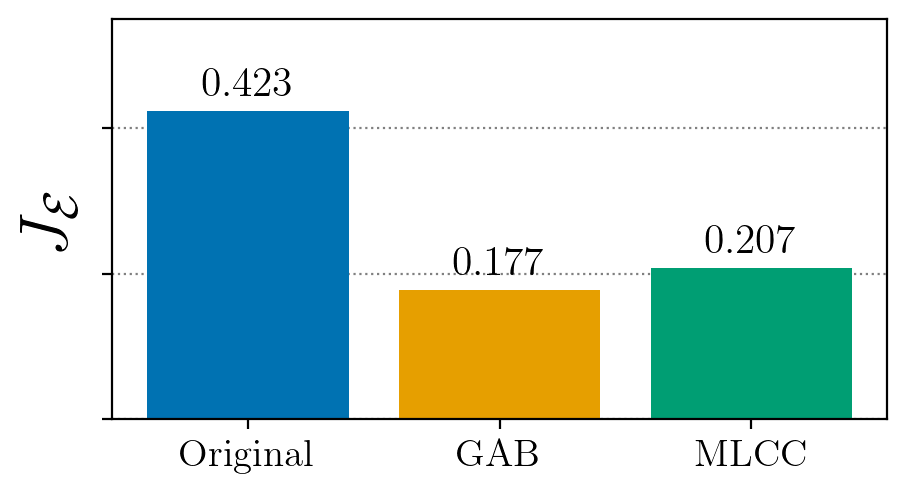
\includegraphics[width=0.95\linewidth]{Images/plot_bar_flows.png}\label{aa}} \\
  
%   \subfloat[Average values]{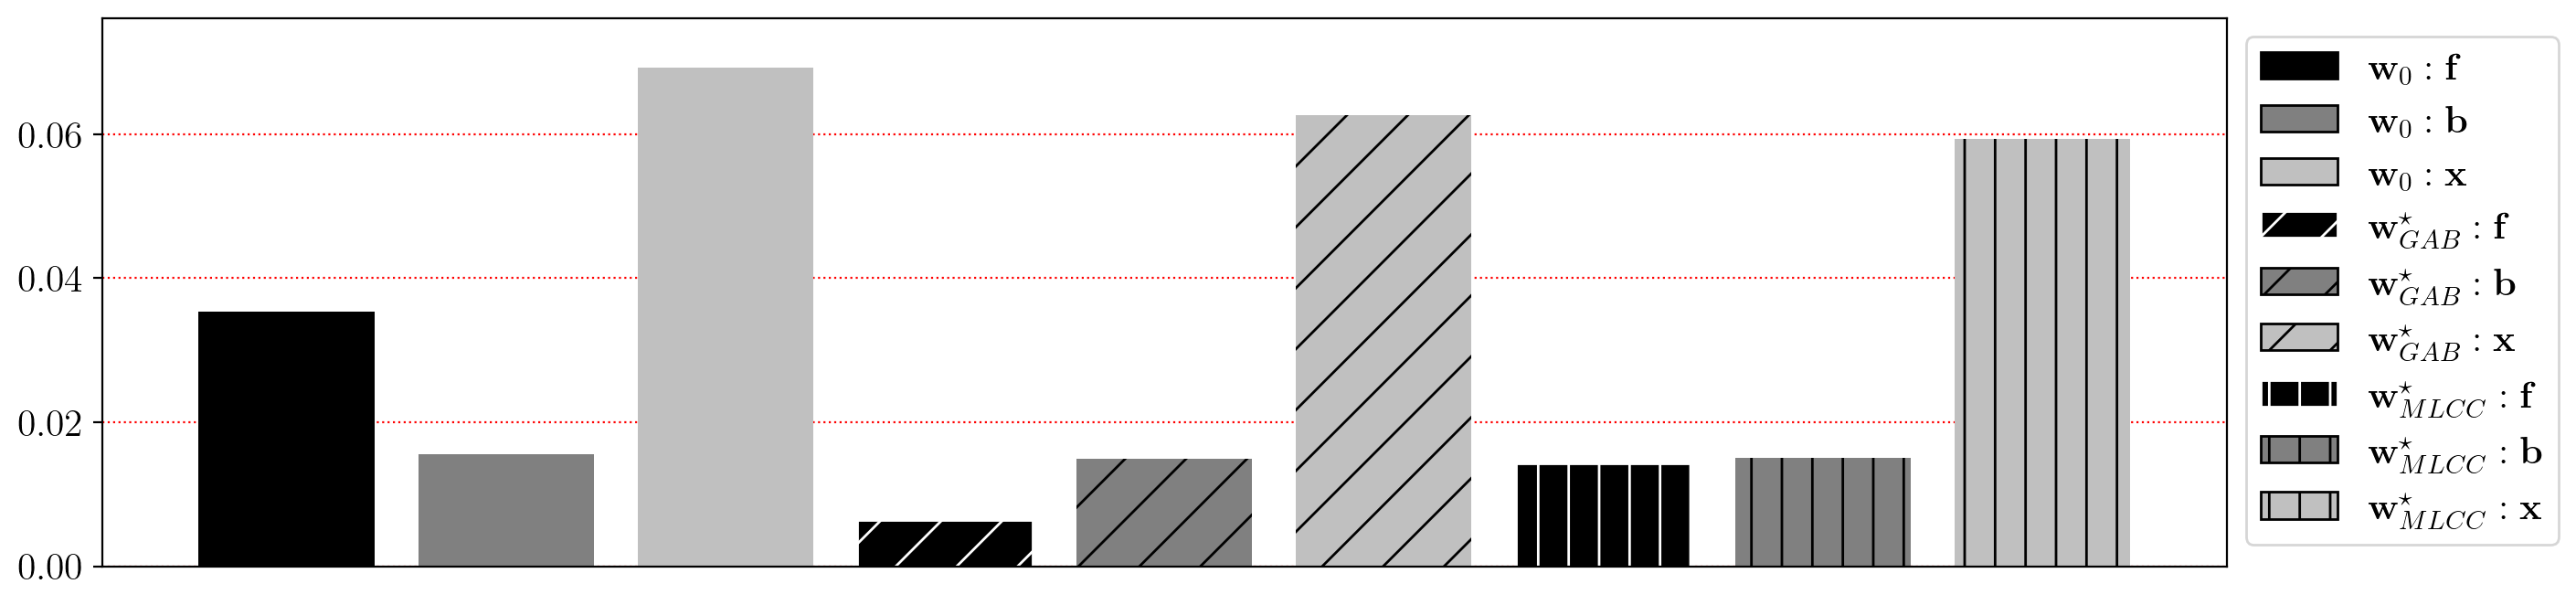
\includegraphics[width=1\linewidth]{Images/plot_bar_average.png}\label{aa_2}}
  
%   \caption{\footnotesize(a) Result of GAB and MLCC algorithms to Problem 1 with a budget of 50\%, i.e., $\alpha=\frac{1}{2}$, (b) Average of traffic factor and bicycle distance and flow, respectively.}
%   \label{bar_plot}
% \end{figure*}

\section{Grenoble Cycling Network Case Study}
\label{study_case}
\begin{figure}[t]
\vspace{0.2cm}
  \centering
 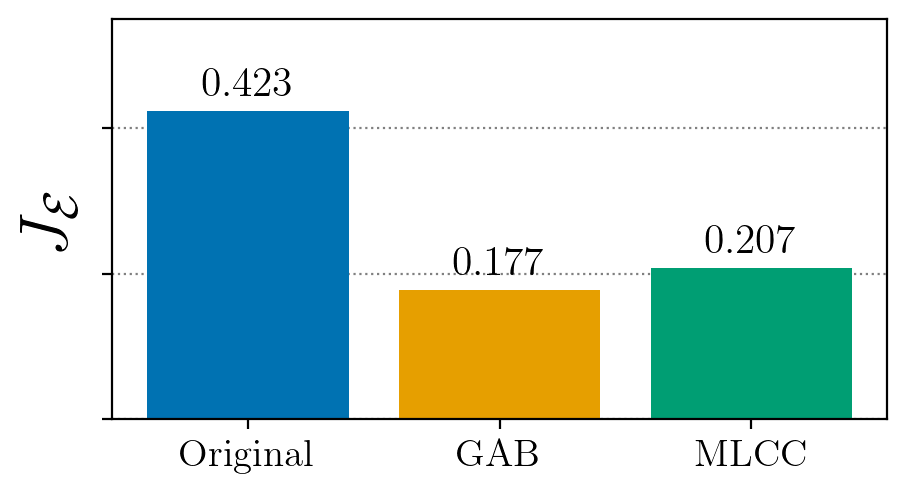
\includegraphics[width=1\linewidth]{Images/plot_bar_flows.png}
  \caption{\footnotesize Initial traffic exposure and reduced exposure after optimization using the GAB and MLCC algorithms for Problem 1 with a budget constraint of 50\%, i.e., $\beta=\frac{1}{2}$.}
  \label{bar_plot}
\end{figure}
\begin{figure*}[t]
\vspace{0.2cm}
  \centering
  \captionsetup[subfigure]{font={footnotesize}, labelfont={footnotesize, bf}, textfont={footnotesize, rm}}

  \subfloat[Original flows]{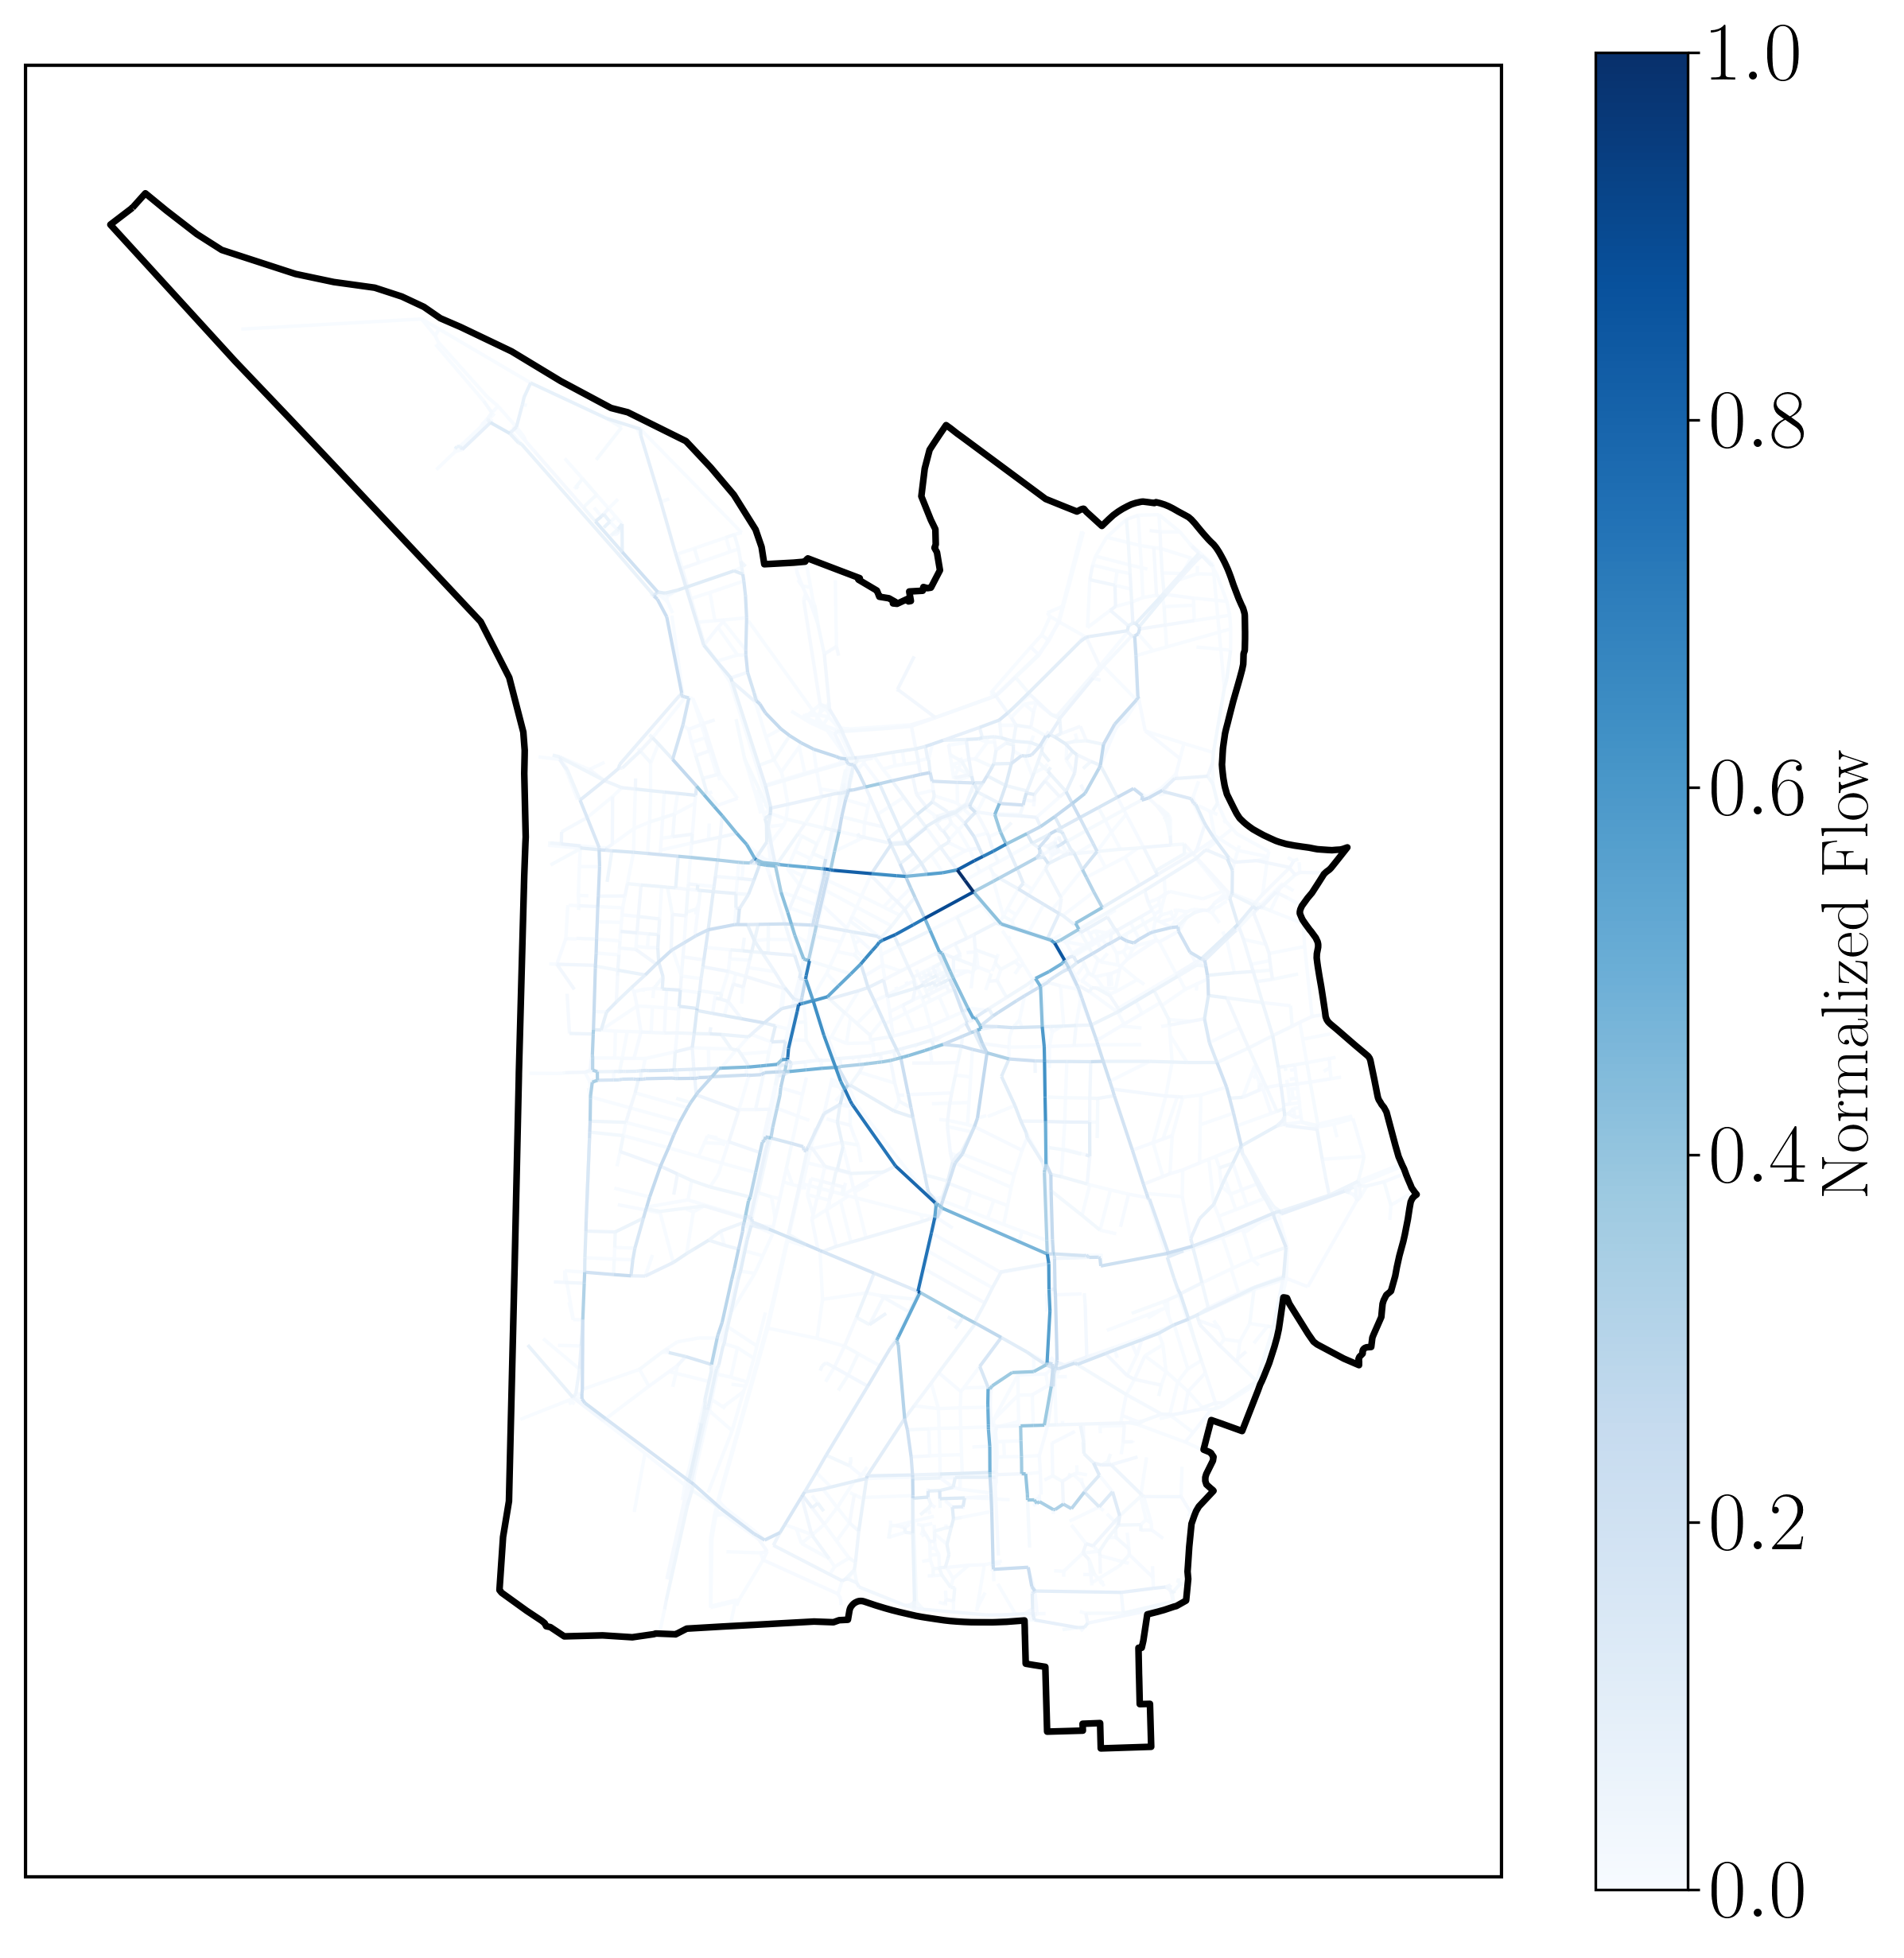
\includegraphics[width=0.31\linewidth]{Images/Grenoble_flows_original.png}\label{ae_1}}
  \hspace{0.004\linewidth} % Adjust horizontal space as 
  \subfloat[GAB flows]{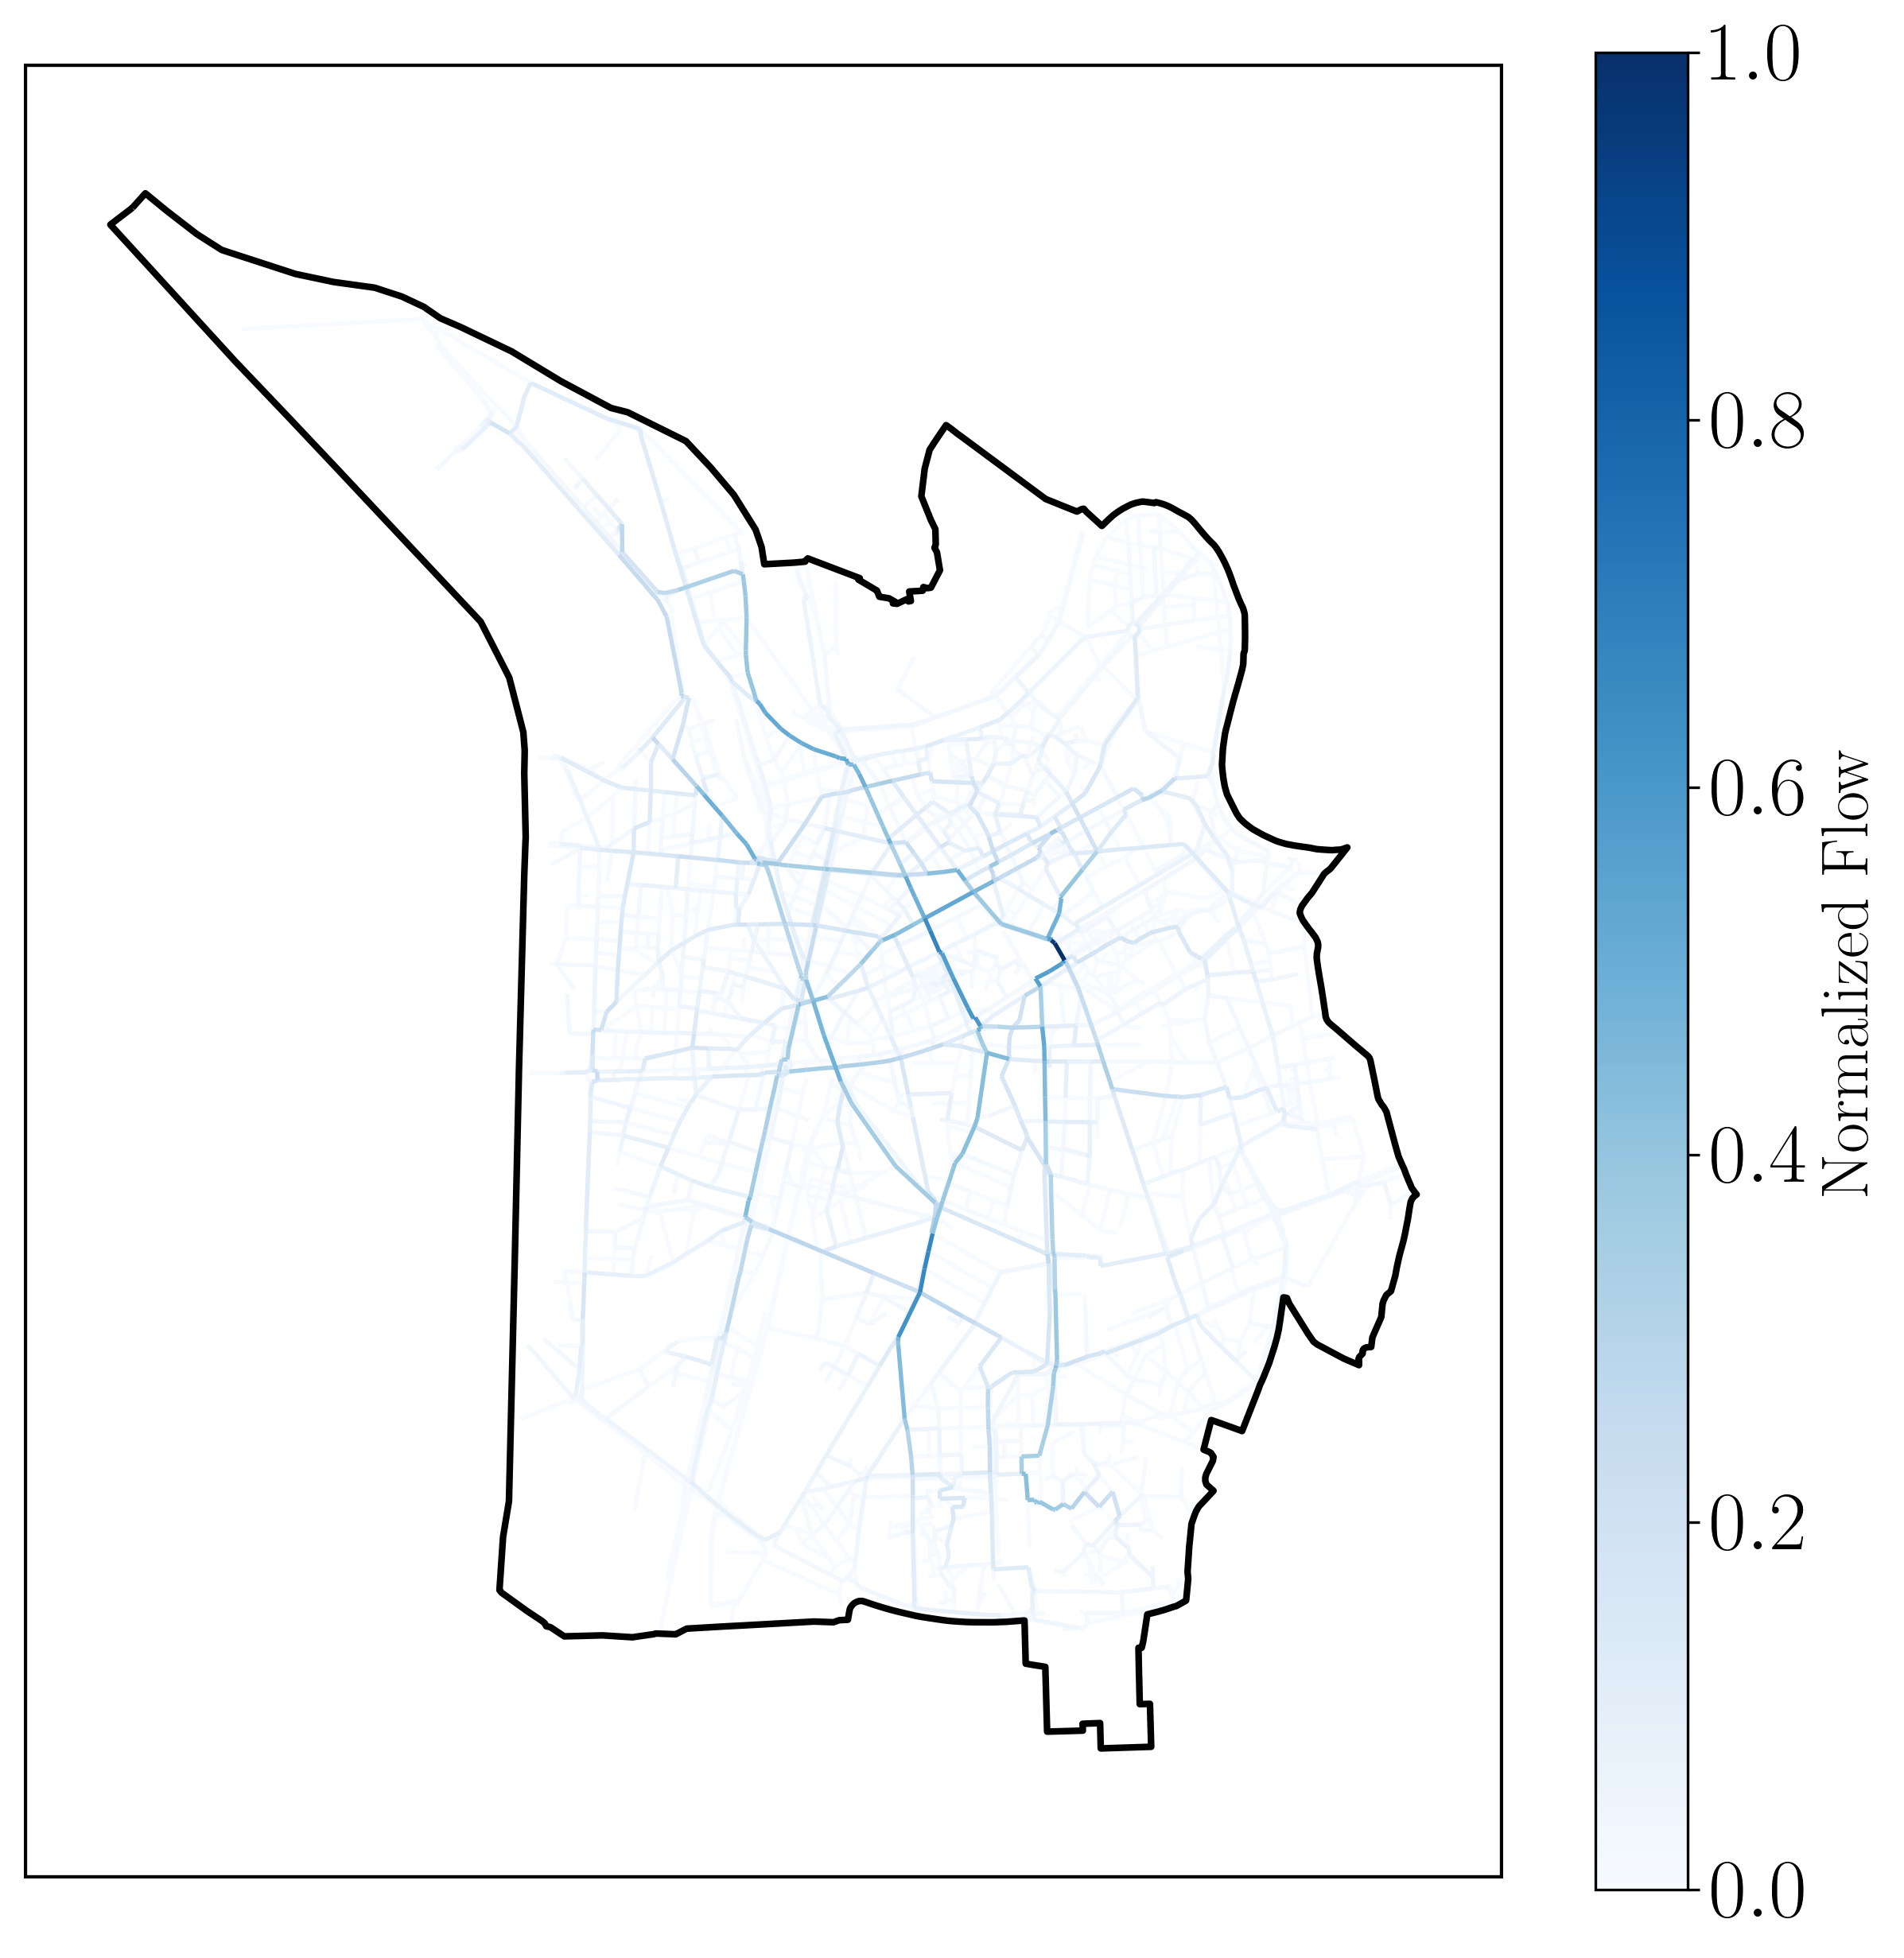
\includegraphics[width=0.31\linewidth]{Images/Grenoble_flows_SGA.png}\label{ae_3}}
  \hspace{0.004\linewidth}
  \subfloat[MLCC flows]{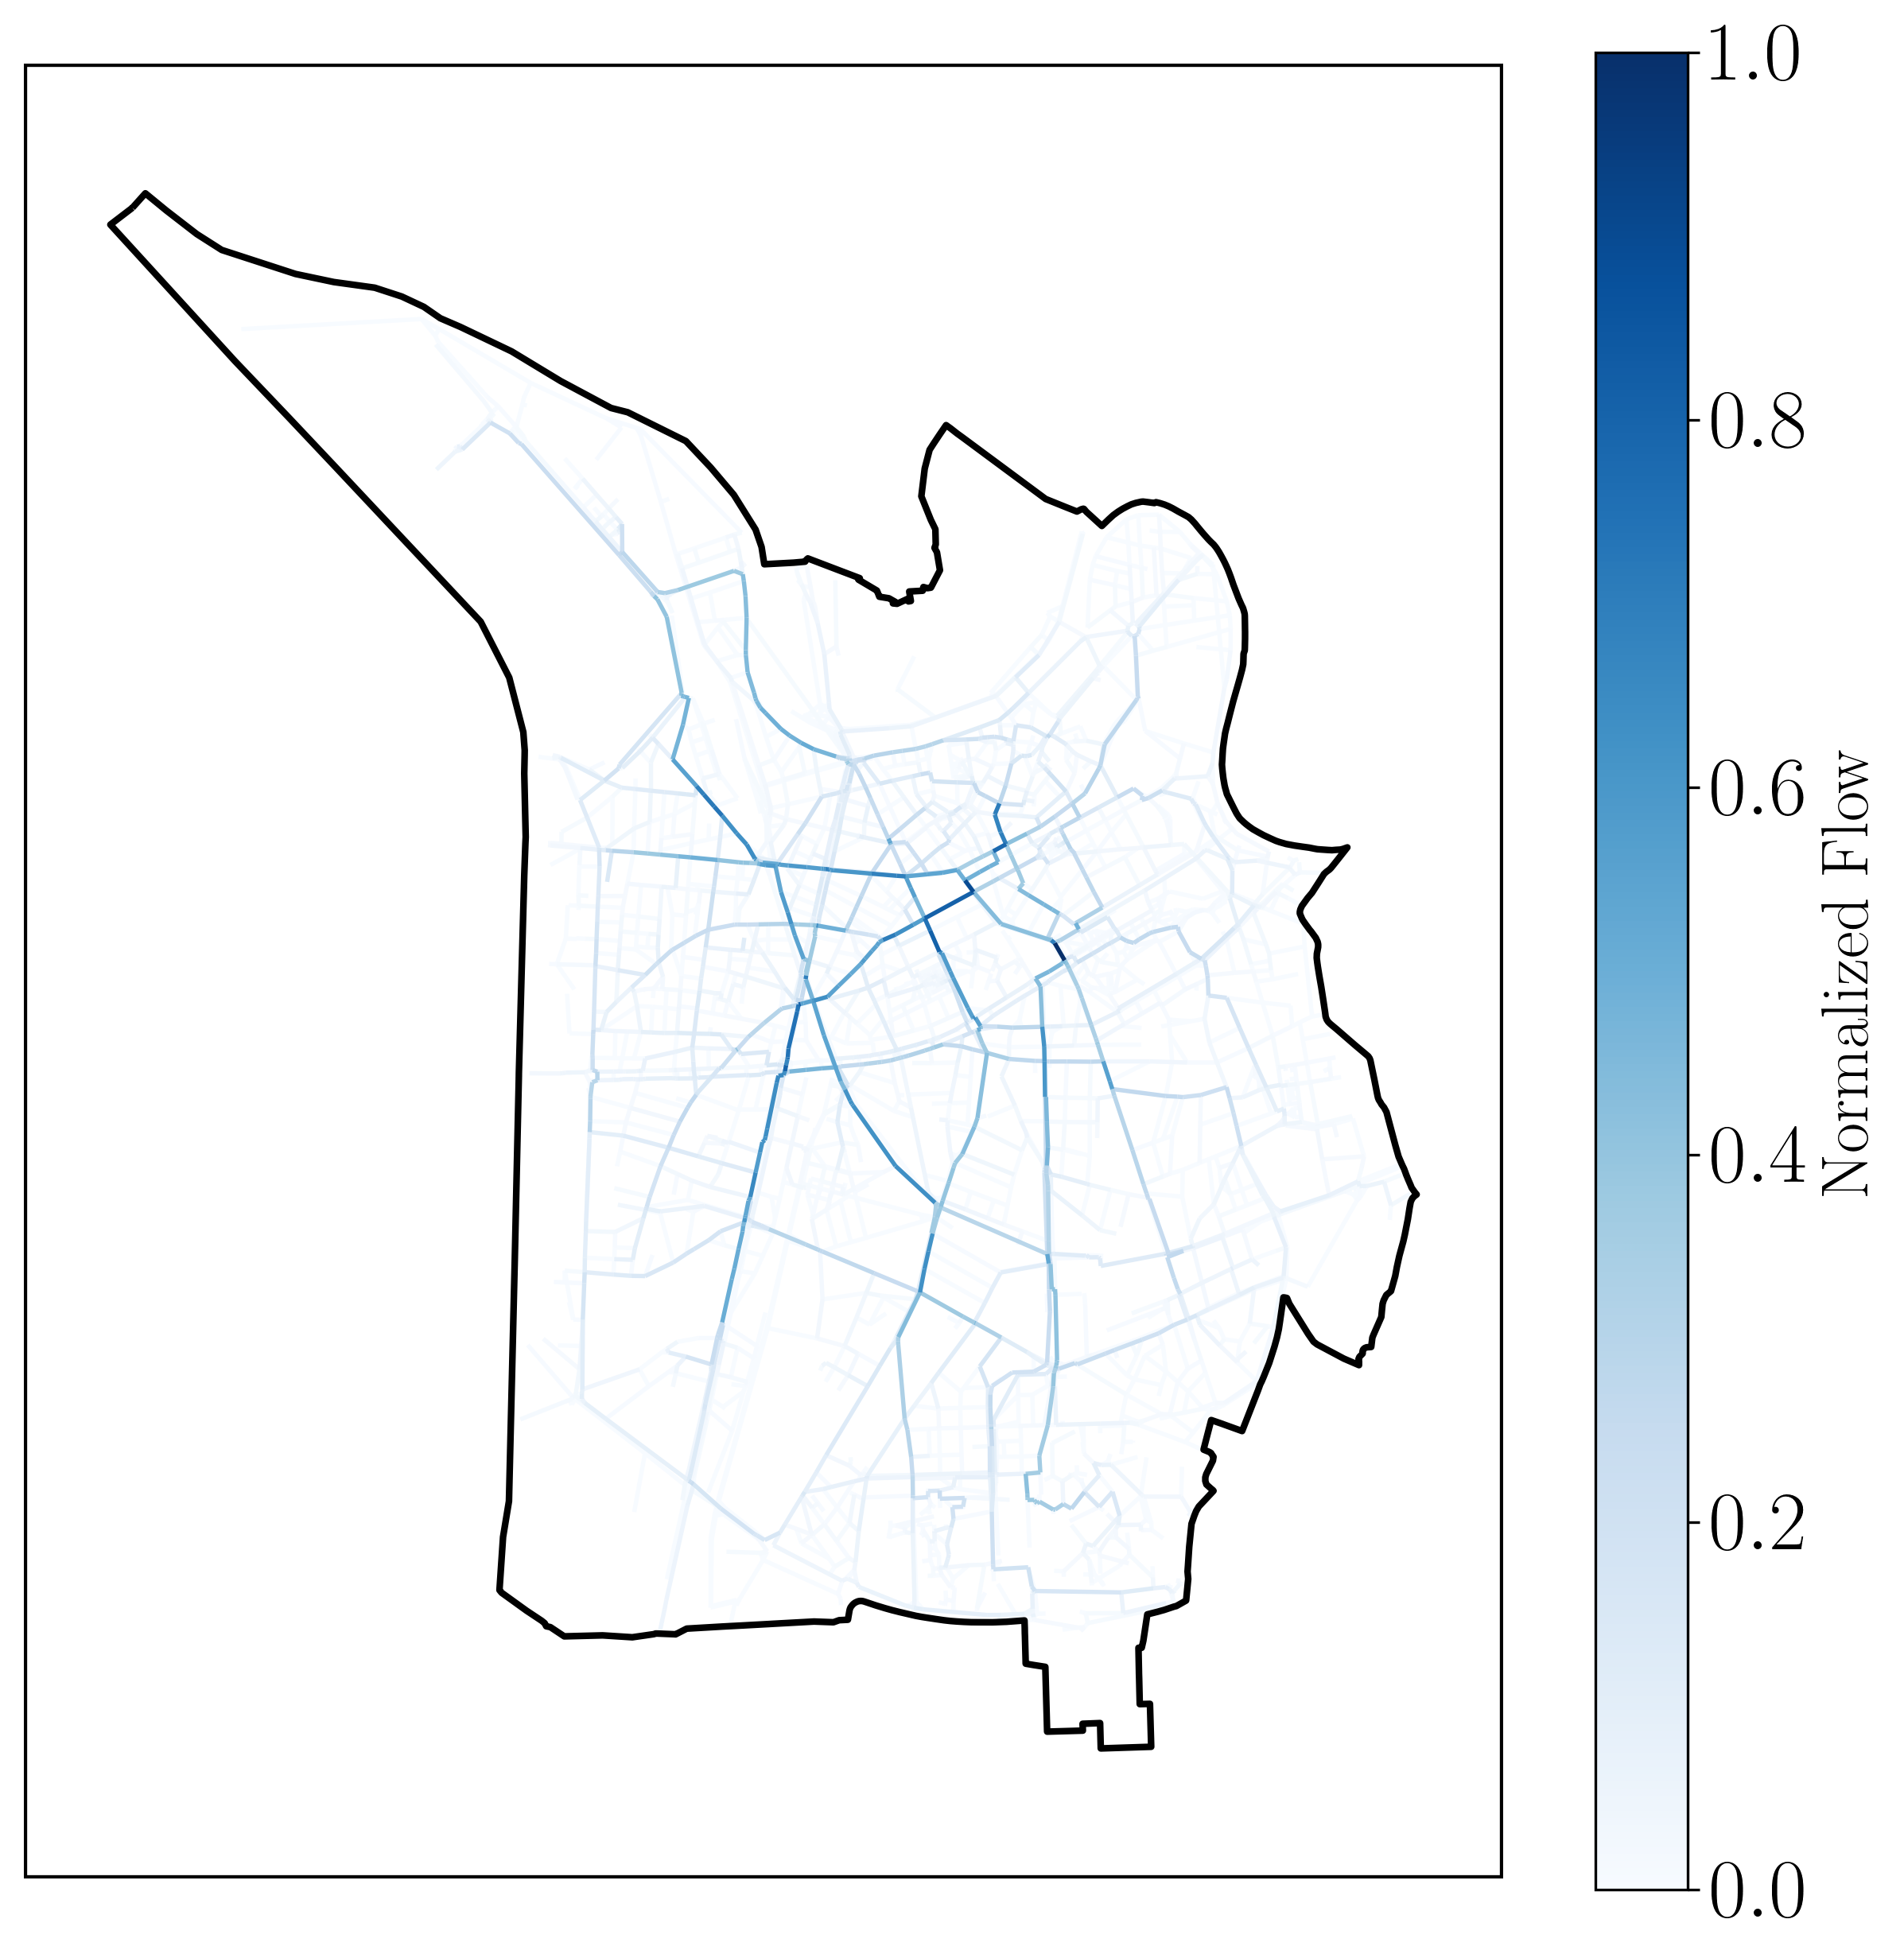
\includegraphics[width=0.31\linewidth]{Images/Grenoble_flows_MLCC.png}\label{ae_5}}\\
  \subfloat[Original DoS]{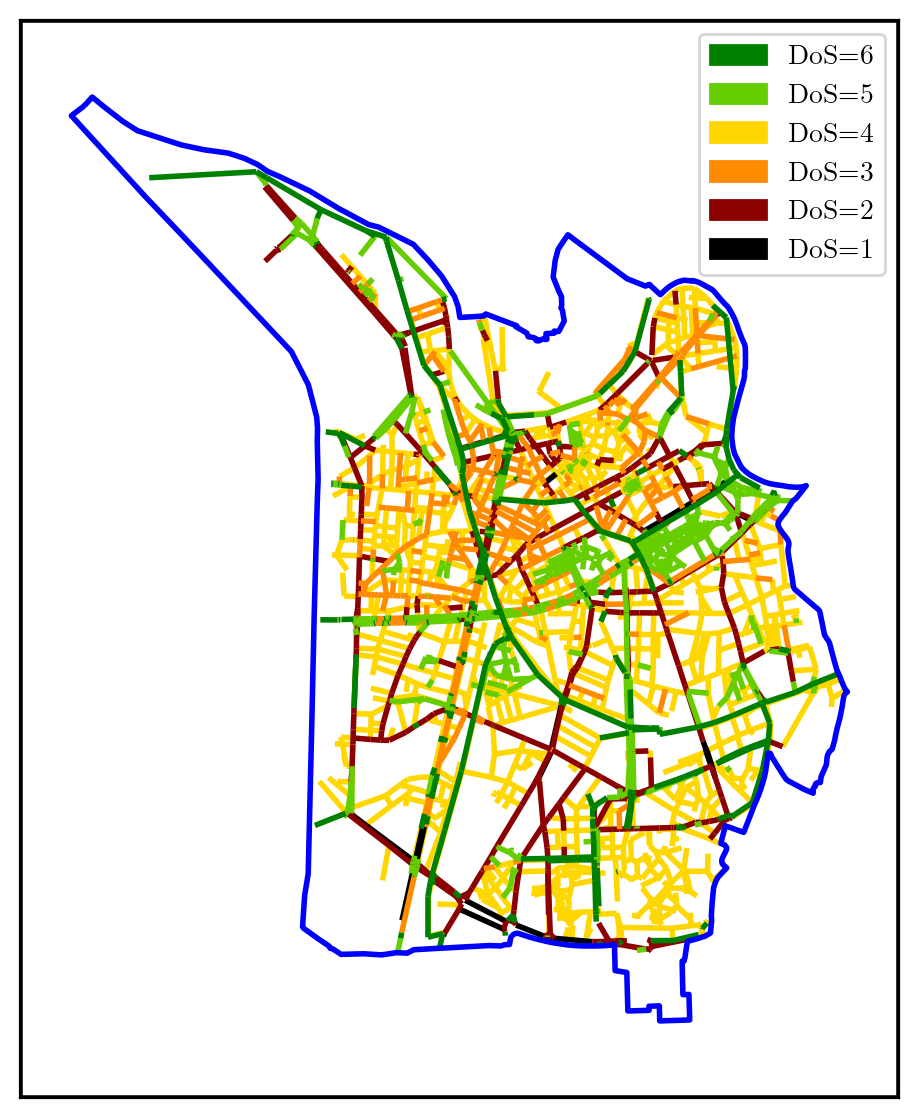
\includegraphics[width=0.26\linewidth]{Images/Grenoble_DOS_original.png}\label{ae_2}}
  \hspace{0.05\linewidth}
   % Adjust horizontal space as needed
  \subfloat[GAB DoS]{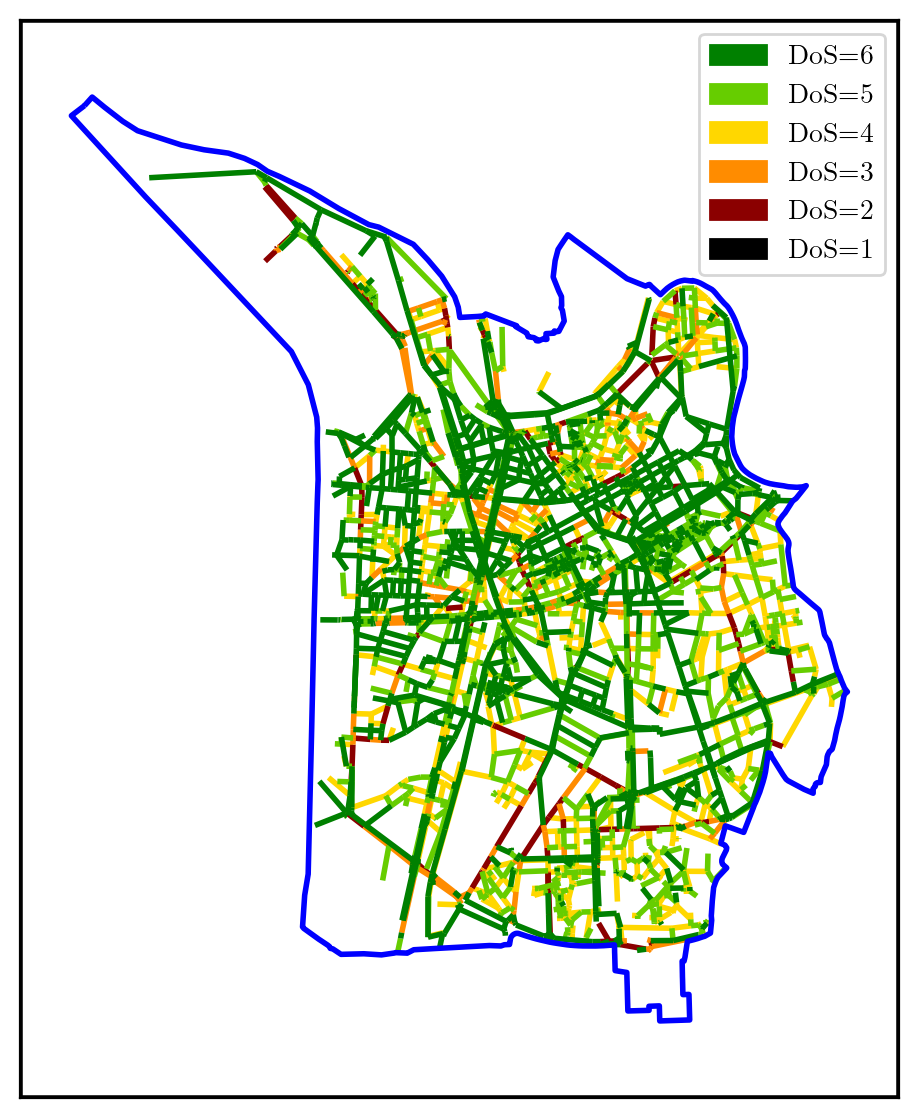
\includegraphics[width=0.26\linewidth]{Images/Grenoble_DOS_SGA.png}\label{ae_4}}
  \hspace{0.05\linewidth}
  % \hspace{0.0045\linewidth} % Adjust horizontal space as needed
  \subfloat[MLCC DoS]{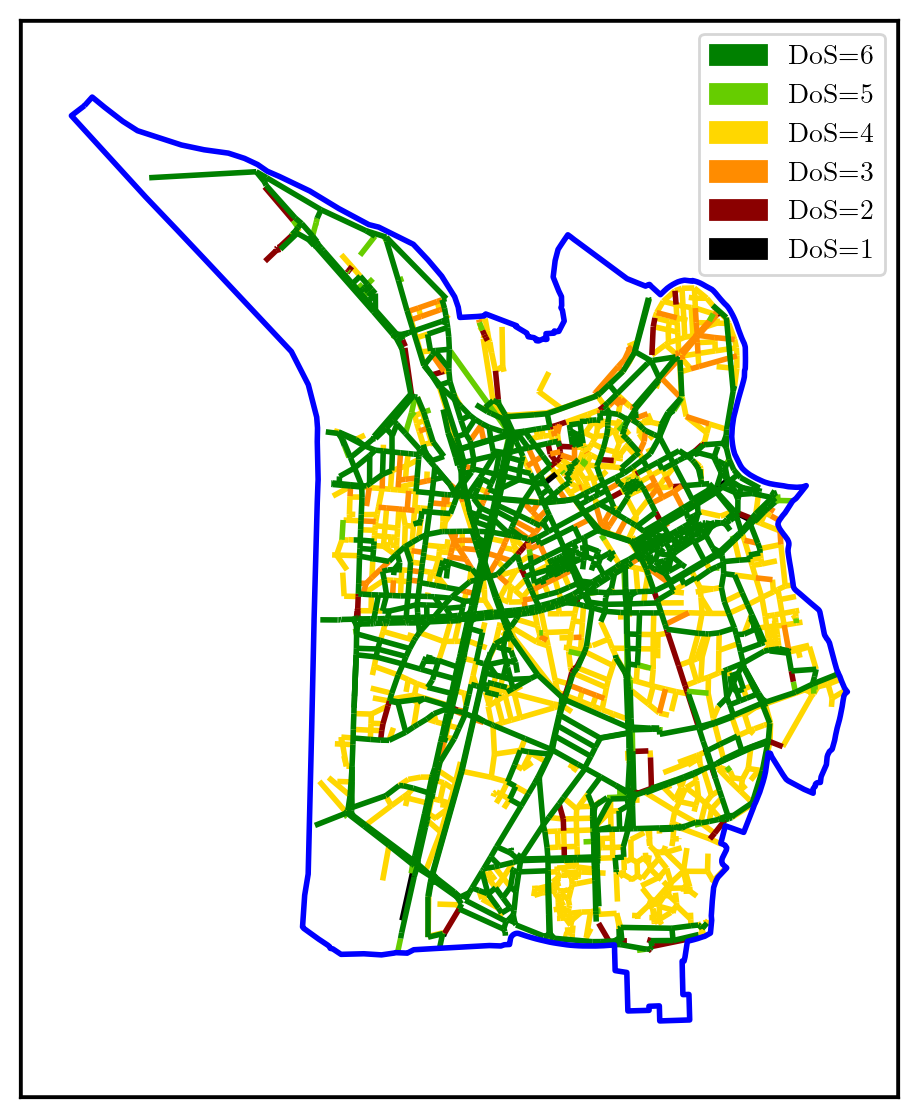
\includegraphics[width=0.26\linewidth]{Images/Grenoble_DOS_MLCC.png}\label{ae_6}}
  \hspace{0.03\linewidth}
  
  \caption{\footnotesize The upper section shows the flow mapping, while the lower section shows the DoS configuration. The optimization algorithms operate with 50\% of the total budget needed for a complete network upgrade. }
  \label{grenoble_case}
\end{figure*}
%%%%%%%%%%%%%%%%%%%%%%%%%%%%%%%%%%%%%%%%%%%%%%%%%%%%%%%%%%%%%%%%%%%%%%%%%%%%%%%%%%%%%%%%%%%%%%%%%%%%%%%%%%%%%%%%%%%%%%%%%%%%%%%%%%%%%%%%%%
In this section, we present the case study of Grenoble, France, and discuss the optimization results achieved by the GAB and MLCC algorithms. We then apply the largest CC metric to compute the overall improvements in perceived safety and comfort resulting from both algorithms.
 \subsection{Parameters and Algorithm Comparisons}
To solve the all-or-nothing traffic assignment problem and determine cyclist flows, as described in Section~\ref{section_flows}, we use parameters that are better suited for the model, as suggested by \cite{cooper2017using}. Specifically, we set $\rho = 0.04$, $\kappa = 0.14$ and $\psi~=~0.84$. The slope factor $s_{a}$ is determined in Table~\ref{table:slope_factors}, where downhill routes are considered as the reciprocal of the slope factor when traversing in the opposite direction.
\begin{table}[h!]
\centering
\begin{tabular}{c|c|c}
\hline
Slope ($m_a$) \% & Uphill Factor ($s_a$) & Downhill Factor ($s_a$) \\ \hline
$m_a < 2$ & 1.0 & 1.0 \\ 
$2 \leq m_a < 4$ & 1.371 & $1/1.371 \approx 0.729$ \\ 
$4 \leq m_a < 6$ & 2.203 & $1/2.203 \approx 0.454$ \\ 
$m_a \geq 6$ & 4.239 & $1/4.239 \approx 0.236$ \\ \hline
\end{tabular}
\caption{\footnotesize Slope factors for cycling distance calculation}
\label{table:slope_factors}
\end{table}
 

 Let $B = \beta \cdot B_{\text{max}}$, be the available budget for optimization, with $B_{\text{max}}$ represents the budget required to upgrade the entire network to DoS $=6$, and $\beta \in \left [ 0,1\right]$. The cost per meter to upgrade the infrastructure along an edge is set to reflect different construction costs between levels, following Cerema's cost \cite{cerema2024_cost} studies. For this analysis, we assume $\beta = \frac{1}{2}$, representing $50$\% of the maximum budget. 

To solve Problem 1, with Algorithm~\ref{pseudocode:GAB} we adapt the standard genetic algorithm from Pygmo \cite{pygmo}. Fig.~\ref{bar_plot} compares the original cyclist exposure to traffic of $0.42$ with the optimized results of $0.17$ and $0.20$ from the GAB and MLCC approaches, respectively. The results demonstrate that GAB is more effective at minimizing traffic exposure compared to MLCC, even though GAB only guarantees a local optimum. As shown in Table \ref{table:dos}, while GAB results in 141 km of bike lanes with DoS=6 and MLCC achieves 170 km, GAB allocates nearly 10 times more bike lanes with DoS=5. This allocation strategy optimizes budget usage by prioritizing a category that is less costly than the highest one while still significantly reducing cyclist exposure to traffic.

Although MLCC does not explicitly consider flow, it still indirectly lowers traffic exposure due to the all-or-nothing traffic assignment model, which assumes cyclists follow the shortest path based on the cyclist distance metric \eqref{cyclist_distance}. This metric heavily depends on the DoS of each lane, and MLCC specializes in connecting origin-destination pairs with high DoS lanes, providing safe and comfortable paths.

\begin{table}[h!]
\centering
\begin{tabular}{c|c|c|c|c|c|c}
\hline
DoS (Km) & 6 & 5 & 4 & 3 & 2 & 1 \\ \hline
Original & 31.0 & 43.9 & 146.9 & 36.3 & 43.8 & 5.9 \\
GAB & 141.8 & 74.0 & 59.0 & 19.9 & 13.2 & 0 \\
MLCC & 170.5 & 6.1 & 105.3 & 16.3 & 7.9 & 1.2 \\ \hline
\end{tabular}
\caption{\footnotesize Number of kilometers of bike lanes for each DoS}
\label{table:dos}
\end{table}

% Fig. \ref{grenoble_case} further illustrates the DoS levels of the network and the distribution of cyclist flows before and after optimization. It is evident that both algorithms effectively upgraded the network, redistributing cyclists and enhancing overall connectivity. This redistribution reduces the use of only a few specific routes and promotes more efficient and safer routes through the network. Future work will focus on further optimizing and enhancing overall perceived safety and comfort while accounting for flow distribution and additional factors, such as potential cyclist congestion. Additionally, we aim to develop an algorithm that can approach the global optimum more closely.
Fig.~\ref{grenoble_case} shows the DoS levels and cyclist flow distribution before and after optimization. Both algorithms effectively upgrade the network, improving connectivity and promoting safer, more efficient routes. Future work will refine optimization, consider cyclist congestion, and develop algorithms closer to the global optimum.
% Now, we use the largest CC metric in \eqref{lcc} to asses overall perceived safety and comfort, we visualize the original levels of perceived safety and comfort compared to those achieved by the GAB and MLCC algorithms. Fig. \ref{perceived_safety_and_comfort} displays the results,  showing a significant increase in perceived safety and comfort compared to the original value of 0.12. The GAB algorithm achieves a global perception score of approximately 0.40, while the MLCC algorithm reaches nearly 0.58. This difference can be attributed to GAB allocating part of the budget to upgrade lanes that are not connected to other high-DoS lanes, whereas connecting safe and comfortable roads is crucial for enhancing perceived safety and comfort within a cycling network.

%Despite not being explicitly designed to maximize overall perceived safety and comfort, GAB performs effectively, and both algorithms significantly improve overall perceived safety and comfort. 
% \begin{figure}[t]
%     \centering
%     \vspace{0.2cm}
% 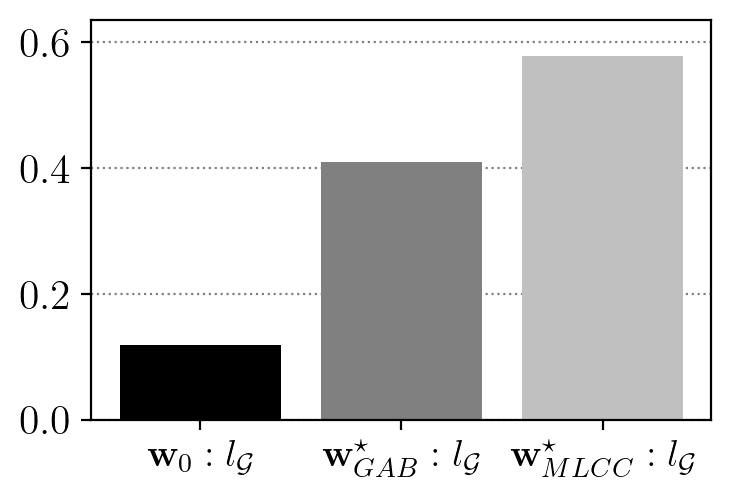
\includegraphics[width=1\columnwidth]{Images/plot_bar_perceived_safety_and_comfort.png}
%     \caption{\footnotesize Global measure of perceived safety and comfort.}
%     \label{perceived_safety_and_comfort}
% \end{figure}




%%%%%%%%%%%%%%%%%%%%%%%%%%%%%%%%%%%%%%%%%%%%%%%%%%%%%%%%%%%%%%%%%%%%%%%%%%%%%%%%%%%%%%%%%%%%%%%%%%%%%%%%%%
% \begin{figure}[t]
%     \centering
% % 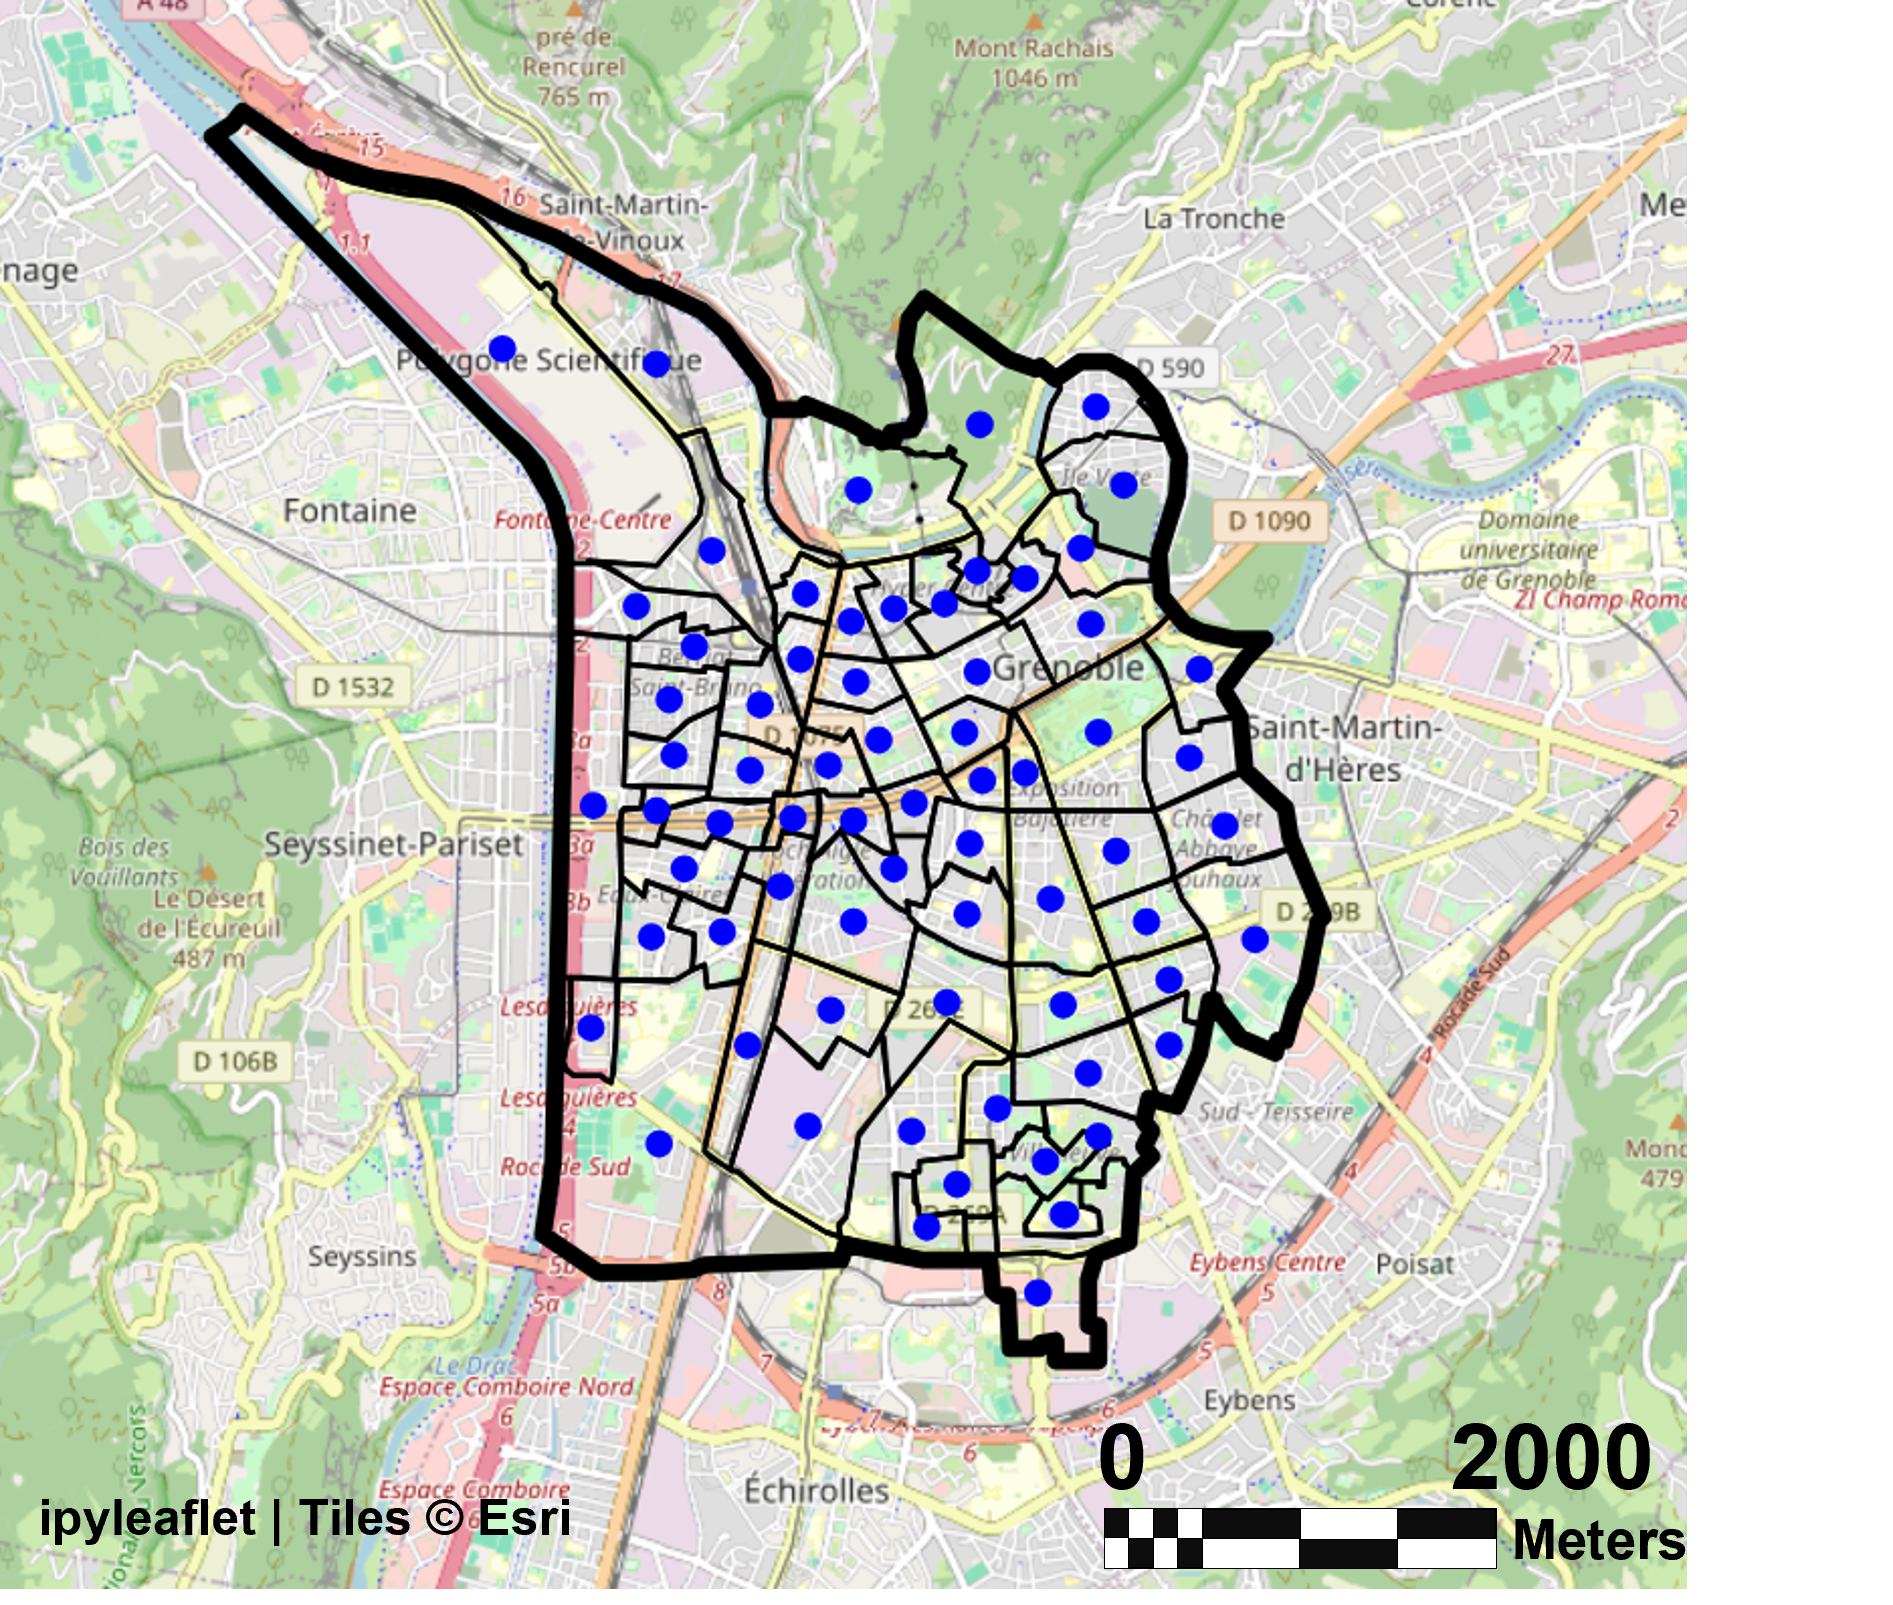
\includegraphics[width=\columnwidth]{Images/Grenoble_O_D.png}
% 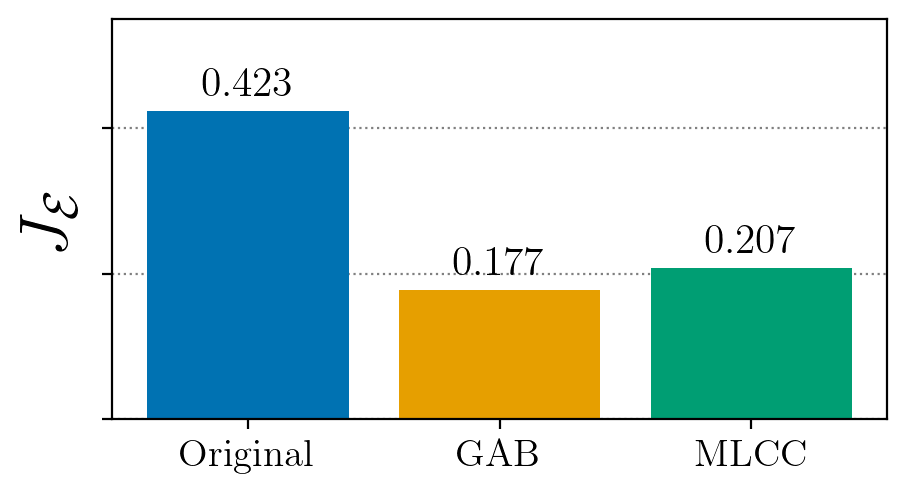
\includegraphics[width=1.1\columnwidth]{Images/plot_bar_flows.png}
%     \caption{\footnotesize Result of bilevel optimization problem with a budget of 50\%}
%     \label{bar_plot}
% \end{figure}

\section{Conclusions}
\label{conclusions}

This work presented a framework for upgrading cycling infrastructure to enhance safety and comfort within budget constraints. Using a genetic algorithm to efficiently allocate resources and an algorithm to improve connectivity among the safest routes, we show that targeted upgrades reduce cyclists' exposure to traffic and improve flow distribution. 
%The frameworks effectively increase perceived safety and comfort both locally and overall in the cycling network.

Future work will focus on taking into account factors such as potential congestion and lane capacity, as well as the impact on other road users, possibly in intermodal settings~\cite{wollenstein2021routing}. In addition to upgrading infrastructure, we aim to integrate justice considerations into the optimization process to ensure the equitable distribution of safety and comfort enhancements across the network~\cite{salazar2024accessibility}.

\section*{Ackwnoledgements}
We thank Dr.\ I.\ New, G. Ganassoli, G. Gasnier and Ir.\ S.\ Betancur Giraldo for proofreading this paper. The authors thank the IDEX for funding M.C.J  mobility  grant. This work was done in collaboration with Project FORBAC under the reference ANR-23-PEPR-002.




% \begin{table*}[h!]
% \centering
% \begin{tabular}{|l|l|l|l|l|}
% \hline
% \textbf{Source Name} & \textbf{Function} & \textbf{Data Type} & \textbf{Reference} \\ \hline
% Geovelo             & Categorizes bike lanes by separation level & Infrastructure classification & \cite{2024graphbased} \\ \hline
% CycleRAP            & Provides crash risk scores & Safety and comfort scoring & \cite{cyclerap2024} \\ \hline
% GTLVille            & Estimates AADT and mean speed near bike paths & Traffic and speed data & \cite{gtlville2024} \\ \hline
% EMD2020             & Surveys general mobility patterns & Household mobility data & \cite{SMMAG_EMD} \\ \hline
% Cerema              & Provides bicycle trip distribution based on distance & Mode choice probability & \cite{cerema2024mobility} \\ \hline
% \end{tabular}
% \caption{Summary of Data Sources Used in the Cycling Network Model. All the data used is open.}
% \label{table:data_sources}
% \end{table*}


%%%%%%%%%%%%%%%%%%%%%%%%%%%%%%%%%%%%%%%%%%%%%%%%%%%%%%%%%%%%%%%%%%%%%%%%%%%%%%%%%%%%%%%%%%%%%%%%%%%%%%%%%%


% \section{Basic safety/comfort accessibility definition}

% Let $p_{(u, \mathcal{C})}$ denote the shortest path from node $u$ to $\mathcal{C}$ (where $\mathcal{C}$ is the largest connected component in Degree of Safety (DoS) level 6). Let $t_{(u, \mathcal{C})}$ represent the travel time along path $p_{(u, \mathcal{C})}$, with $t_{\text{max}}$ as the time threshold beyond which accessibility to the safest and most comfortable connected component $\mathcal{C}$ starts to decrease.

% We define the safety/comfort inaccessibility of a node $u \in \mathcal{V}$ as the additional travel time beyond the threshold required to reach $\mathcal{C}$, given by:

% \begin{equation}
% \mu_{u} = \max \left\{ 0, \frac{t_{(u, \mathcal{C})} - t_{\text{max}}}{t_{\text{max}}} \right\}.
% \end{equation}

% Here, $\mu_{u}$ is zero if the travel time $t_{(u, \mathcal{C})}$ is below the threshold $t_{\text{max}}$, and it is positive if the travel time exceeds this threshold.

% The average regional safety/comfort inaccessibility for each region $r \in \mathcal{R}$ is defined as the weighted average of the extra time for each region, weighted by the frequency of occurrence:

% \begin{equation}
% \mu^{r} = \frac{\sum_{u \in \mathcal{V}^{r}} q_{u} \cdot \mu_{u}}{\sum_{u \in \mathcal{V}^{r}} q_{u}}.
% \end{equation}
% \begin{equation}
% \mu_{u}^{\delta} = 
%      \begin{cases}
%          \max \left \{ 0, 1 - \frac{\delta_{(u, \mathcal{C})}}{\delta^{\text{total}}_{(u, \mathcal{C})}} \right \} & \text{if } \delta^{\text{total}}_{(u, \mathcal{C})} > 0, \\
%          0 & \text{if } \delta^{\text{total}}_{(u, \mathcal{C})} = 0,
%      \end{cases}
% \end{equation}


% Finally, the overall inaccessibility of node $u \in \mathcal{V}$ is defined as:
% \begin{equation}
% \mu_{u} = \frac{1}{2} \left( \mu_{u}^{\delta} + \mu_{u}^\top \right).
% \end{equation}

% \begin{equation}
%      \mu_{u} = \frac{1}{2} \left( \underset{\mu_{u}^{\delta}}{\underbrace{\max  \left \{ 0, 1 - \frac{\delta_{(u, v)}}{\delta^{\text{total}}_{(u,v)}} \right \}}}  + \underset{\mu_{u}^\top}{\underbrace{\max \left \{ 0, \frac{t_{(u,v)}-t_{\text{thd}}}{t_{\text{max}}-t_{\text{thd}}} \right \}}}  \right),
% \end{equation}



%%%%%%%%%%%%%%%%%%%%%%%%%%%%%%%%%%%%%%%%%%%%%%%%%%%%%%%%%%%%%%%%%%%%%%%%%%%%%%%%%%%%%%%%%%%%%%%%%%%%%%%%%%
%%%%%%%%%%%%%%%%%%%%%%%%%%%%%%%%%%%%%%%%%%%%%%%%%%%%%%%%%%%%%%%%%%%%%%%%%%%%%%%%%%%%%%%%%%%%%%%%%%%%%%%%%%
% \noindent\textbf{Problem: Network-upgrade optimization problem (Congestion bike lanes priority)}
% \begin{align}
%     \label{problem_a_1}
%     w^{\star} &= \;   \underset{\tilde{w} \in \Omega}{\operatorname{argmax}} \; \left (  ||\hat{y}_{w_{0}}- \hat{y}(\tilde{w}) || + \mathcal{C} +J_{\text{acc}} \right )\\
%     &= \label{problem_a_2} \;  \underset{\tilde{w} \in \Omega}{\operatorname{argmax}} \; \left ( ||(M_{w_{0}}- M_{\tilde{w}}) \theta^{\star} || + \mathcal{C} +J_{\text{acc}} \right ),\\
%     & \text{s.t. } (15)-(16) \text{ \& } (24).
% \end{align}


%%%%%%%%%%%%%%%%%%%%%PSEUDOCODE
% {\color{blue}
% Let $a=(u,v) \in \mathcal{A}$, we define $\eta_{a} = 1-\min \left \{ \mu_{u}, \mu_{v} \right \}$
% \noindent\textbf{Problem: Network-upgrade optimization problem (High 
% flow and inaccessibility bike lanes priority)}
% \begin{align}
%     \label{problem_a_1}
%     w^{\star} &= \;   \underset{\tilde{w} \in \Omega}{\operatorname{argmax}} \; \left (\sum_{a=1}^{|\mathcal{A}|} x_{a}\cdot |\hat{y}(\tilde{w}_{a})-\hat{y}_{w_{0,a}}| \cdot \frac{1}{\left ( \eta_{a} + 1 \right )}  \right )\\
%     &= \label{problem_a_2} \;  \underset{\tilde{w} \in \Omega}{\operatorname{argmax}} \; \left ( \sum_{a=1}^{|\mathcal{A}|} x_{a} \cdot |(M_{\tilde{w}_{a}}-M_{w_{0,a}}) \theta^{\star} | \cdot \frac{1}{\left ( \eta_{a} + 1 \right )}   \right ),\\
%     & \label{problem_a_3} \text{under} \quad   \sum_{a=1}^{|\mathcal{A}|} d_{a} \cdot \pi(w_{a},\tilde{w}_{a}) \leq B.
% \end{align}

% The pseudocode refers to the MLCC algorithm to solve the problem. Steps correspond to the different items.

% \floatname{algorithm}{Algorithm}
% \begin{algorithm}[ht]
% \caption*{MLCC Algorithm} 
% \label{edges_upgrade_pseudocode}
% \footnotesize
% \begin{algorithmic}[1]
% \State \textbf{Input:} Original graph: $\mathcal{G}$. Budget: $B$.
% \State \textbf{Output:} $\mathcal{G}$ with edges upgraded.
% \For{$C$ \textbf{in} set of CCs of $\mathcal{G}$}

% \State $\mathcal{G}_{C} \gets (V(\mathcal{G}_{C}), E(\mathcal{G}_{C}), W(\mathcal{G}_{C}))$ induced graph by $C$
% \State $\gamma \gets \max{ \left \{ \omega_{e} \colon e \in E(\mathcal{G}_{C}) \right \} }$
% \State list\_$\mathcal{G}_{C} \gets \left \{ C_{\gamma} \colon C_{\gamma} \text{ is a connected subgraph } \right.$
% \State $\quad $ (see Section~\ref{connected_component})  \Comment{{\color{gray} Step 1.1 }} 
% \State $C_{\hat{\gamma}} \gets \max{ \left \{ \text{list\_}\mathcal{G}_{C} \right \}}$
% \If{$\gamma < 6$}
%         \State Upgrade Subgraph($C_{\hat{\gamma}}, B$)
%     \EndIf
% \If{$\gamma == \max{ \left \{ \omega_{e} \colon e \in E(C_{\hat{\gamma}}) \right \}}$}
%         \For{$C_{\tilde{\gamma}}$ \textbf{in} $\text{sorted(list\_}\mathcal{G}_{C}) $}
%         \State Connect Graphs($C_{\hat{\gamma}}, C_{\tilde{\gamma}}, B$) \Comment{{\color{gray} Step 1.2 }} 
% \EndFor
% \EndIf
% \For{$\tilde{\gamma} \gets 5$ \textbf{to} $2$}
%         \State $\text{list\_}\mathcal{G}_{C_{\tilde{\gamma}}} \gets \left \{ C_{\tilde{\gamma}} \colon C_{\tilde{\gamma}} \text{ is a connected subgraph} \right \}$ 
%         \State $\quad \quad \quad \quad \quad$ (see Section~\ref{connected_component})
%         \For{$C_{\tilde{\gamma}}$ \textbf{in} $\text{sorted(list\_}\mathcal{G}_{C_{\tilde{\gamma}}})$} \Comment{{\color{gray} Step 2 }} 
%         \State Connect Graphs ($C_{\hat{\gamma}}, C_{\tilde{\gamma}}, B$) 
%         \State Upgrade Subgraph($C_{\tilde{\gamma}}, B$)
% \EndFor
% \EndFor
% \EndFor
% \end{algorithmic}
% \end{algorithm}
% %Connected graphs $C_{\gamma}$ and $C_{\tilde{\gamma}}$ are constructed using the same criteria as defined in the $l_{\mathcal{G}}$ metric. They are sorted to arrange their elements in descending order based on the total geographical length of their edges.


% \floatname{algorithm}{Function}
% \begin{algorithm}[H]
% \caption*{Connect Graphs}
% \label{pseudocode:connect_graphs}
% \footnotesize
% \begin{algorithmic}[1]
% \State \textbf{Input:} Graphs: $\mathcal{G}_{1}$ and $\mathcal{G}_{2}$. Budget: $B$.
% \State \textbf{Output:} Upgrade the DoS of DoS shortest path between $\mathcal{G}_{1}$ and $\mathcal{G}_{2}$ so that all its edges have the maximum possible DoS value.
% \For{$e$ \textbf{in} shortest DoS path between $\mathcal{G}_{1}$ and $\mathcal{G}_{2}$}
% \For{$i \gets 6$ \textbf{to} $2$}
%     \If{$B \geq d_{e} \cdot \pi(\omega_{e}, i)$ \textbf{and} $i > \omega_{e}$}
%         \State $\omega_{e} \gets i$
%         \State $B \gets B-d_{e} \cdot \pi(\omega_{e}, i)$
%     \Else
%         \State \textbf{end Main Algorithm}
%     \EndIf
% \EndFor
% \EndFor
% \end{algorithmic}
% \end{algorithm}

% \floatname{algorithm}{Function}
% \begin{algorithm}[H]
% \caption*{Upgrade Subgraph}
% \label{pseudocode:upgrade_subpgraph}
% \footnotesize
% \begin{algorithmic}[1]
% \State \textbf{Input:} Subgraph: $\mathcal{H}$. Budget: $B$.
% \State \textbf{Output:} $\mathcal{H}$ with edges upgraded at the maximum possible DoS value.
% \For{$e$ \textbf{in} edges of $\mathcal{H}$}
% \For{$i \gets 6$ \textbf{to} $2$}
%     \If{$B \geq d_{e} \cdot \pi(\omega_{e}, i)$ \textbf{and} $i > \omega_{e}$}
%         \State $\omega_{e} \gets i$
%         \State $B \gets B-d_{e} \cdot \pi(\omega_{e}, i)$
%     \Else
%         \State \textbf{end Main Algorithm}
%     \EndIf
% \EndFor
% \EndFor
% \end{algorithmic}
% \end{algorithm}
% }


% Given a fixed budget $B$. We introduce the following notations:

% \begin{itemize}
%     \item $w_{0} = \left [ w_{1}, \ldots, w_{a}, \ldots, w_{|\mathcal{A}|} \right ]$ are the original arc weights \CRD of the graph $\mathcal{G}$ to be optimized.
%     \item $\tilde w = \left [ \tilde{w}_{1},  \ldots, \tilde{w}_{a}, \ldots,\tilde{w}_{|\mathcal{A}|} \right ] \in \Omega $ are the candidate weights to be optimized, with,
%     \begin{equation} \nonumber
%         \Omega = \left \{ \tilde{w} \in \mathbb{N}^{|\mathcal{A}|} \colon w_{a} \leq \tilde{w}_{a} \leq w_{\text{DoS}_{6}},  \forall a \in \left \{1,2, \ldots, |\mathcal{A}| \right \}  \right\}.
%     \end{equation} 
% \end{itemize}
% Based on the linear model structure derived above and the identified parameters, we can now define two predicted model outputs, each with different DoS weights,
% \begin{equation*}
%  \hat{y}_{w_{0}} = M_{w_{0}} \theta^{\star}, \quad \quad \hat{y}(\tilde{w}) = M_{\tilde{w}}\theta^{\star}
% \end{equation*}
%   with $M_{w_{0}} \in~\mathbb{R}^{2 \times 4}$, and $M_{\tilde{w}} \in~\mathbb{R}^{2 \times 4}$ are matrices defined as:
% \begin{equation} \nonumber
%     M_{w_{0}} = 
%     \begin{bmatrix}
%         m_{w_{0}} & 0\\ 
%         0 & m_{w_{0}}
%             \end{bmatrix} , \quad \quad 
%         M_{\tilde{w}} = \begin{bmatrix}
%         m_{\tilde{w}} & 0\\ 
%         0 & m_{\tilde{w}}
%     \end{bmatrix}
% \end{equation}
% with $m_{w_{0}}$ and $m_{\tilde{w}}$ in $\mathbb{R}^{1 \times 2}$, 
% $$
% m_{w_{0}} = \left[   1,  l_{\mathcal{G}} \right ],  \quad \quad m_{\tilde{w}} = \left[   1,  l_{\mathcal{G}_{\tilde{w}}} \right ]
% $$
% where $l_{\mathcal{G}_{\tilde{w}}}$ is computed in $\mathcal{G}$ with the \CRD changed to $\tilde{w}$. Denoting $\pi(w_{a},\tilde{w}_{a})$ the cost or price per meter of upgrading arc $a$ from $w_{a}$ to $\tilde{w}_{a}$, and let $\mathbf{x} \in \mathbb{R}_{\geq 0}^{|\mathcal{A}|}$ the vector of all the flows, then the optimization problem can now be formulated as follows:


% \noindent\textbf{Problem: Network-upgrade optimization problem}
% \begin{align}
%     \label{problem_a_1}
%     \omega^{\star} &= \; \underset{\tilde{\omega} \in \Omega}{\operatorname{argmax}} \; ||\hat{y}_{\omega_{0}}- \hat{y}(\tilde{\omega}) || \\
%     w^{\star} &= \;  \underset{\tilde{w} \in \Omega}{\operatorname{argmax}} \; \left ( (M_{\tilde{w}}-M_{w_{0}}) \theta^{\star} \right ),\\
%     & \label{problem_a_3} \text{under} \quad   \sum_{a=1}^{|\mathcal{A}|} d_{a} \cdot \pi(w_{a},\tilde{w}_{a}) \leq B.
% \end{align}
% \noindent\textbf{Problem: Network-upgrade optimization problem (High 
% flow bike lanes priority)}
% \begin{align}
%     \label{problem_a_1}
%     w^{\star} &= \;   \underset{\tilde{w} \in \Omega}{\operatorname{argmax}} \; \left (\sum_{a=1}^{|\mathcal{A}|} x_{a} \cdot |\hat{y}(\tilde{w}_{a})-\hat{y}_{w_{0,a}}| \right )\\
%     &= \label{problem_a_2} \;  \underset{\tilde{w} \in \Omega}{\operatorname{argmax}} \; \left ( \sum_{a=1}^{|\mathcal{A}|} x_{a} \cdot |(M_{\tilde{w}_{a}}-M_{w_{0,a}}) \theta^{\star} | \right ),\\
%     % &= \label{problem_a_2} \;  \underset{\tilde{w} \in \Omega}{\operatorname{argmax}} \; \left ( \mathbf{x} \cdot (M_{\tilde{w}_{a}}-M_{w_{0}}) \theta^{\star} \right ),\\
%     & \label{problem_a_3} \text{under} \quad   \sum_{a=1}^{|\mathcal{A}|} d_{a} \cdot \pi(w_{a},\tilde{w}_{a}) \leq B.
% \end{align}










\bibliographystyle{unsrt}
\bibliography{mybibfile}






\end{document}